% =====================================================================
%  Results chapter: architecture, optimiser, and paradigm through the
%  tangent kernel. UNIFIED draft.
%
%  Supersedes the split between the earlier kernel draft (message
%  passing in the JASTROW) and results_backflow.tex (message passing in
%  the BACKFLOW): both are the same relational-channel idea seen through
%  the tangent kernel, and are merged here. All numbers are on the
%  thesis ansatz at DMC-quality energies; seed counts are stated.
% =====================================================================
\graphicspath{{../results/figures/results/}{../results/figures/results/kernel/}{../results/figures/}}
\chapter{Architecture, optimisation and sampling}
\label{ch:kernel}

The previous chapter showed that the ansatz works: it reaches reference quality wherever it was
compared with a reference, and the states it produces carry the staged Wigner-molecule structure the
diagnostics were built to detect. Why the solver can represent those states, and what
governs whether they can be trained at all, are separate and harder questions.

Three observations from that chapter remain unexplained. Two networks of the same size,
trained the same way and landing on the same energy, need not be the same object. A
natural-gradient step that is decisive in one training regime does nothing in another. And
an importance-sampled objective reproduces a Markov chain's answer in one corner of the
phase diagram and departs from it in the next.

All three can be examined through the per-sample, column-centred log-derivative matrix
\begin{equation}
  O_{ki} \;=\; \frac{\partial \log|\Psi_{\btheta}(\bx_k)|}{\partial \theta_i},
  \qquad k=1,\dots,B,\;\; i=1,\dots,P,
  \label{eq:kernel-O}
\end{equation}
and on its two Gram matrices, the quantum geometric tensor $S = O^{\!\top}O / B$ and the
neural tangent kernel $K = OO^{\!\top}$~\cite{JacotEtAl2018-NTK,StokesEtAl2020-QuantumNaturalGradient}.
That gives the chapter its structure:

\begin{quote}
\emph{Architecture} determines the shape of the tangent space.\\
The \emph{optimiser} acts on it through its metric.\\
The \emph{sampling measure} determines how well that metric can be estimated.
\end{quote}

\noindent The chapter takes them in that order. The instrument throughout is the \emph{effective dimension} of the tangent space---the
participation ratio of the QGT spectrum $\{\lambda_a\}$,
\begin{equation}
  d_{\mathrm{eff}}(S) \;=\; \frac{\left(\sum_a \lambda_a\right)^2}{\sum_a \lambda_a^2},
  \label{eq:deff}
\end{equation}
which counts how many directions actually carry Fisher weight, whatever the parameter
count says. Beside it sit the local-energy variance $\Var(E_L)$, zero only for an exact
eigenstate; the effective sample size; and the condition number $\kappa(S)$, which is
reported in \S\ref{sec:kernel-cond} and turns out to be large everywhere and therefore
diagnostic of nothing by itself.

Architectures are compared on a common probe set---the same configurations for every model,
never each model's own $|\Psi|^2$---and below $\omega=0.1$ every relative error is measured
against our own converged variational energies, so it reports internal consistency rather
than accuracy. The tooling is anchored on the analytic two-electron ground state, where the
ansatz returns $E=3.000127$~Ha ($+0.004\%$) at squared overlap $1.000000$.

% =====================================================================
\section{Message passing and the variational geometry}
\label{sec:kernel-q1}

How do the implemented message-passing and separable model families differ after training?
We ask this separately of the correlator and the backflow. The Slater reference, analytic
cusp and training protocol are shared, but the correlators use different learned pair
features, and the backflows differ in capacity, coordinate preprocessing and centre-of-mass
projection (\S\ref{sec:bf-init}). The comparisons therefore identify differences between the
archived implementations; they do not isolate message routing alone.

\subsection{The correlator: tangent-space compression}
\label{sec:kernel-q1a}

At $N=6$, $\omega=1$ the two correlators are indistinguishable in energy. Trained to DMC
quality across a $20$k--$164$k parameter ladder, every model lands within $\pm0.1\%$ of the
reference, and the best raw energy belongs to a $164$k separable network---twice the
message-passing parameter count. Both have reached the same observed energy floor at this
resolution. That agreement hides two differences developed below: the message-passing
correlator has lower local-energy variance across the confinement range and, under the
chosen parametrisations, concentrates its tangent weight differently.

Their tangent geometry is not indistinguishable. On a common probe set the message-passing
correlator reaches a reference-quality state in $d_{\mathrm{eff}}\approx1.2$--$1.7$ over three seeds,
where every separable network needs $2.9$--$3.6$; the two sets do not overlap, and their
closest approach is still a factor of $1.7$. Capacity does not close the gap. Scaling the
separable network eightfold, from $20$k to $164$k parameters, moves its effective dimension
only from $3.6$ to $2.9$, and the $89$k network that matches the message-passing one in size
sits at $3.6$. The gap moves by at most $0.26$ whether scored on either family's samples or
on pooled points. With three and four runs respectively, we report the values rather than a
sigma-separation.

\begin{figure}[htbp]\centering
  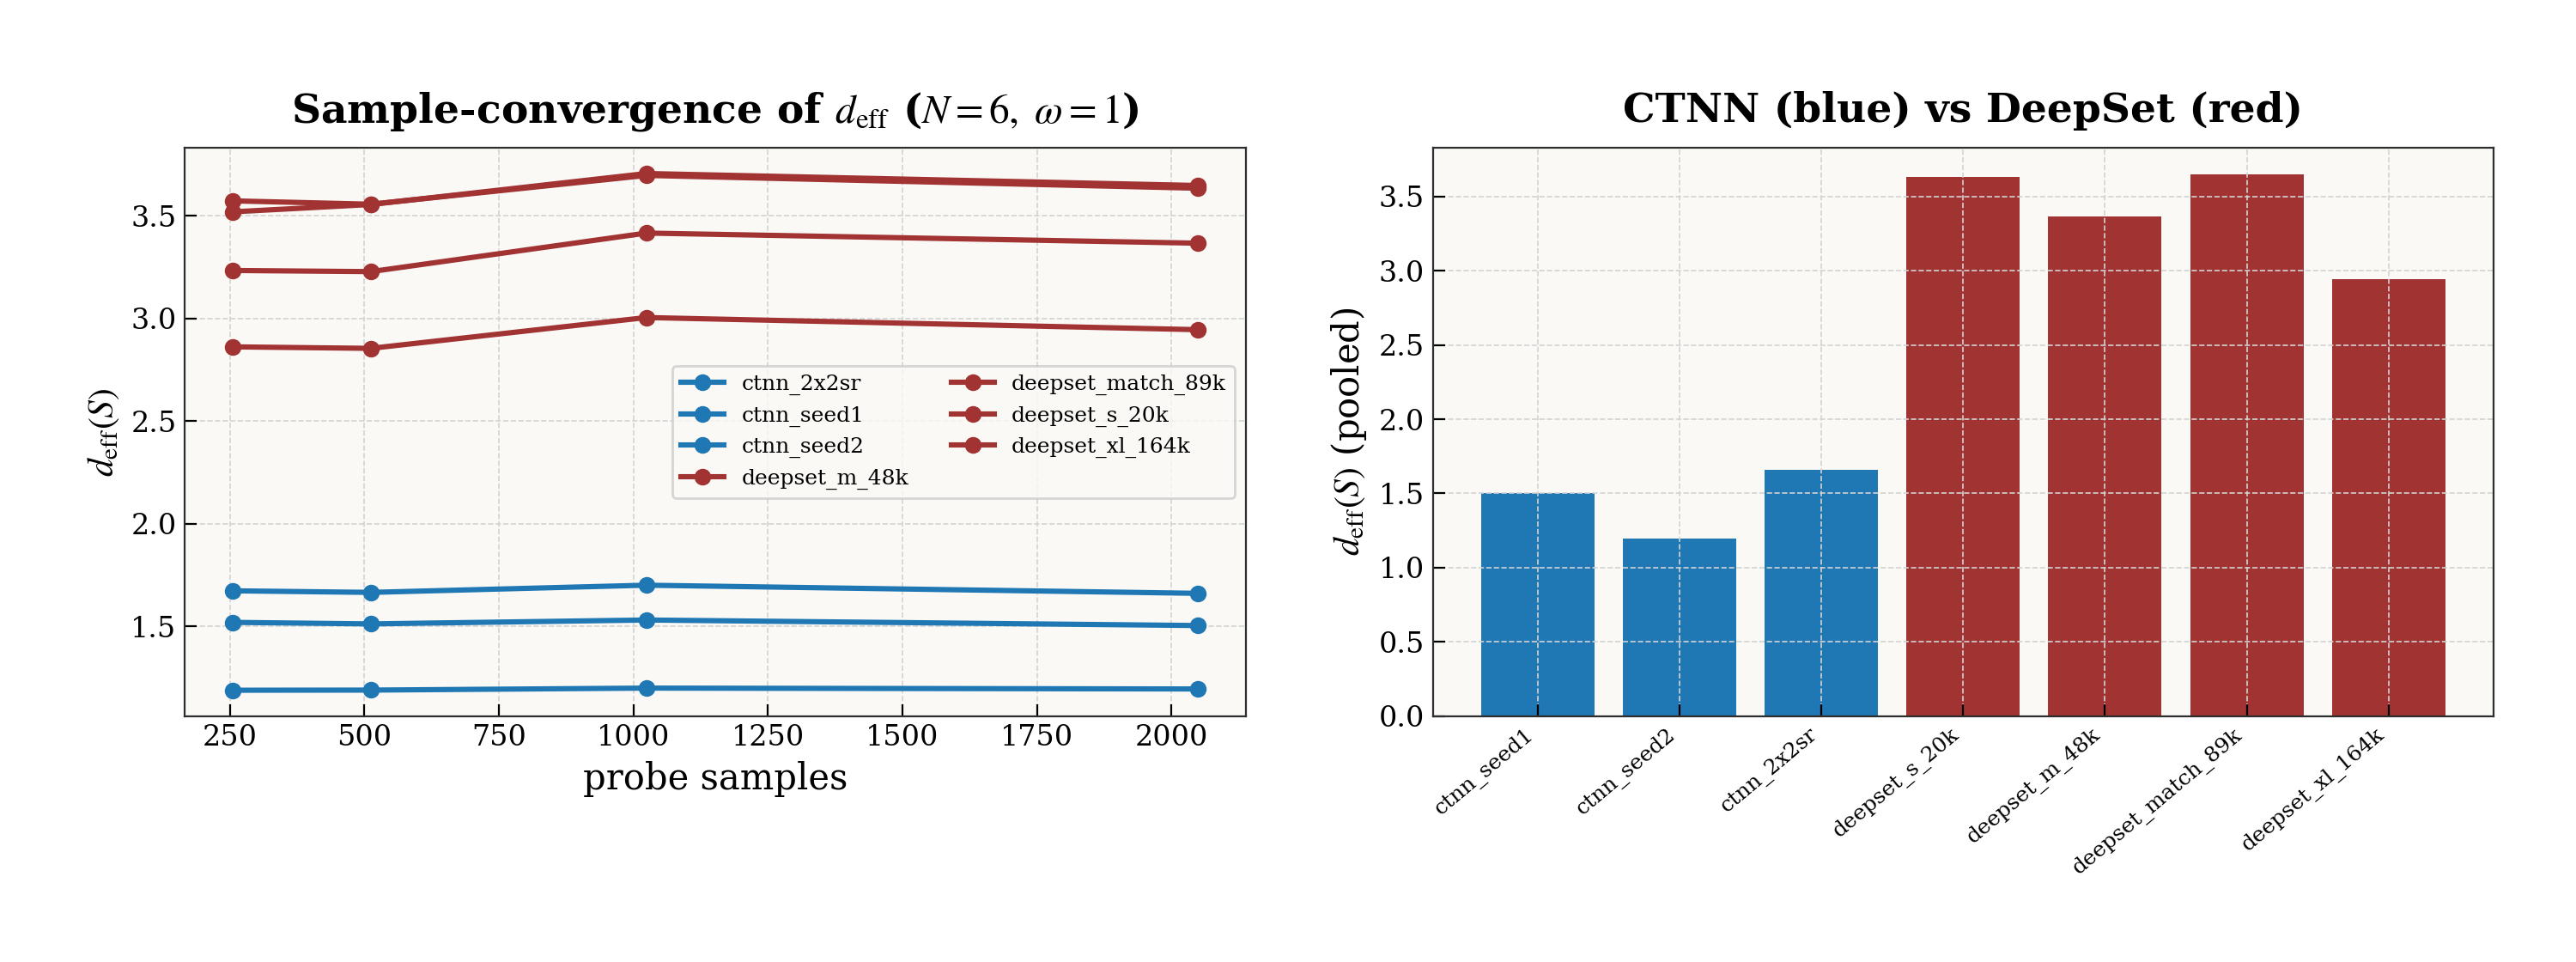
\includegraphics[width=0.95\textwidth]{fair_dimension.png}
  \caption[Message passing concentrates the correlator's Fisher weight]{Effective dimension
  of the correlator's tangent space ($N{=}6$, $\omega{=}1$) on a common pooled probe.
  \emph{Left:} convergence in the number of probe samples. \emph{Right:} per model. The CTNN
  (blue) sits at $d_{\mathrm{eff}}\!\approx\!1.2$--$1.7$ and every DeepSet (red) at
  $\approx\!2.9$--$3.6$; scaling the DeepSet from $20$k to $164$k parameters does not close
  the gap. $d_{\mathrm{eff}}$ depends on the parametrisation (\S\ref{sec:kernel-q1a}).}
  \label{fig:q1a-fairdim}
\end{figure}

The dimension gap is a strong-confinement effect: toward the Wigner crystal both families reach
${\sim}3.7$, although they occupy different tangent subspaces. A single-seed inversion at
the crystal reported in an earlier draft did not survive seeding. Because no backflow is
present here, division of correlation between the correlator and backflow is not at issue.

One more limit applies to every tangent-space quantity in this chapter. The QGT spectrum
depends on the parametrisation: rescaling a layer or changing a normalisation can reweight
tangent directions without changing the state. The result is therefore specific and useful:
under the parametrisations and normalisation conventions used here, the message-passing
correlator concentrates its empirical Fisher weight in fewer directions. It does not show
that the architecture represents the state with intrinsically fewer degrees of freedom.
Only the energy and local-energy variance are state-level comparisons, and only the variance
separates these families.

\paragraph{Local-energy variance.} $d_{\mathrm{eff}}$
stops separating the families at the crystal, and rank will turn out to be gauge-like
(\S\ref{sec:synthesis}). The local-energy variance does neither: it is defined on the
state, vanishes only for an exact eigenstate, and is directly comparable between any two
ansätze evaluated on their own $|\Psi|^2$. Measured at matched training protocol,
$\Var(E_L)$ is lower for the message-passing correlator at every confinement
(Table~\ref{tab:varEL}), by factors between $1.2$ and $3.4$, while the two are
indistinguishable in energy.

At the crystal the three-seed means differ by a factor of $1.8$, rather than the $7.4$
obtained by pairing single best runs. Capacity does not remove the effect: at $\omega=1$ the
capacity-matched $89.4$k separable network widens the ratio to $3.4$. Intermediate
confinements ($\omega=0.28,\,0.05,\,0.03$) preserve the ordering at ratios $1.2$--$1.8$.
The difference is not resolved at the smallest depth-analysis tier ($12$k against $9$k), so
the claim is about trained models at production width, not either architecture at every size.

\begin{table}[htbp]\centering
\caption[Local-energy variance by architecture]{Local-energy variance at $N{=}6$, matched training protocol, both architectures at
reference-quality energy ($|{\rm err}|\le0.13\%$). Lower is better; $\Var(E_L)\to0$ only for
an exact eigenstate. The basis column gives the evidential status of each row: the $\omega=0.01$ row is a
three-seed mean, the rest are single runs of the production cascade. The unseeded rows
establish the ordering, which never reverses, and not the precise factor
(\S\ref{sec:kernel-q1a}). The last row repeats $\omega=1$ against the capacity-matched
$89.4$k separable network.}
\label{tab:varEL}
\begin{tabular}{lcccc}
\hline
$\omega$ & CTNN & DeepSet & ratio & basis \\
\hline
$1.0$  & $1.09\times10^{-2}$ & $2.51\times10^{-2}$ & $2.3$ & single run, $79.8$k vs $47.7$k \\
$0.5$  & $4.62\times10^{-3}$ & $1.01\times10^{-2}$ & $2.2$ & single run, $79.8$k vs $47.7$k \\
$0.1$  & $5.63\times10^{-4}$ & $1.14\times10^{-3}$ & $2.0$ & single run, $79.8$k vs $47.7$k \\
$0.01$ & $1.85\times10^{-5}$ & $3.35\times10^{-5}$ & $1.8$ & 3-seed mean, $79.8$k vs $47.7$k \\
\hline
$1.0$  & $2.75\times10^{-2}$ & $9.38\times10^{-2}$ & $3.4$ & matched, $79.8$k vs $89.4$k \\
\hline
\end{tabular}
\end{table}

\paragraph{Relating the leading tangent directions to selected operators.} At the exact
$N=2$ anchor the selected dictionary describes the leading mode with
$R^2=1.00$, using a breathing mode
($\partial_\omega$), a correlation-hole mode, and the first relative excitation. This is not
special to two bodies. Projecting the leading tangent mode of trained correlators onto a
dictionary of selected operators (breathing/monopole, quadrupole, correlation-hole,
pair-linear), seed-averaged over well-trained checkpoints (energy within $1.5\%$ of
reference), the CTNN reaches $R^2\!\gtrsim\!0.93$ at $N=6$ and $R^2\!\approx\!1.00$ at $N=12$
across the whole confinement range $\omega\in[0.01,1]$, and both architectures reproduce the
$N=2$ naming at strong confinement (Fig.~\ref{fig:mode-naming}). For the message-passing
correlator, the direction carrying most of the tangent weight is well described by this small
dictionary.

\begin{figure}[htbp]\centering
  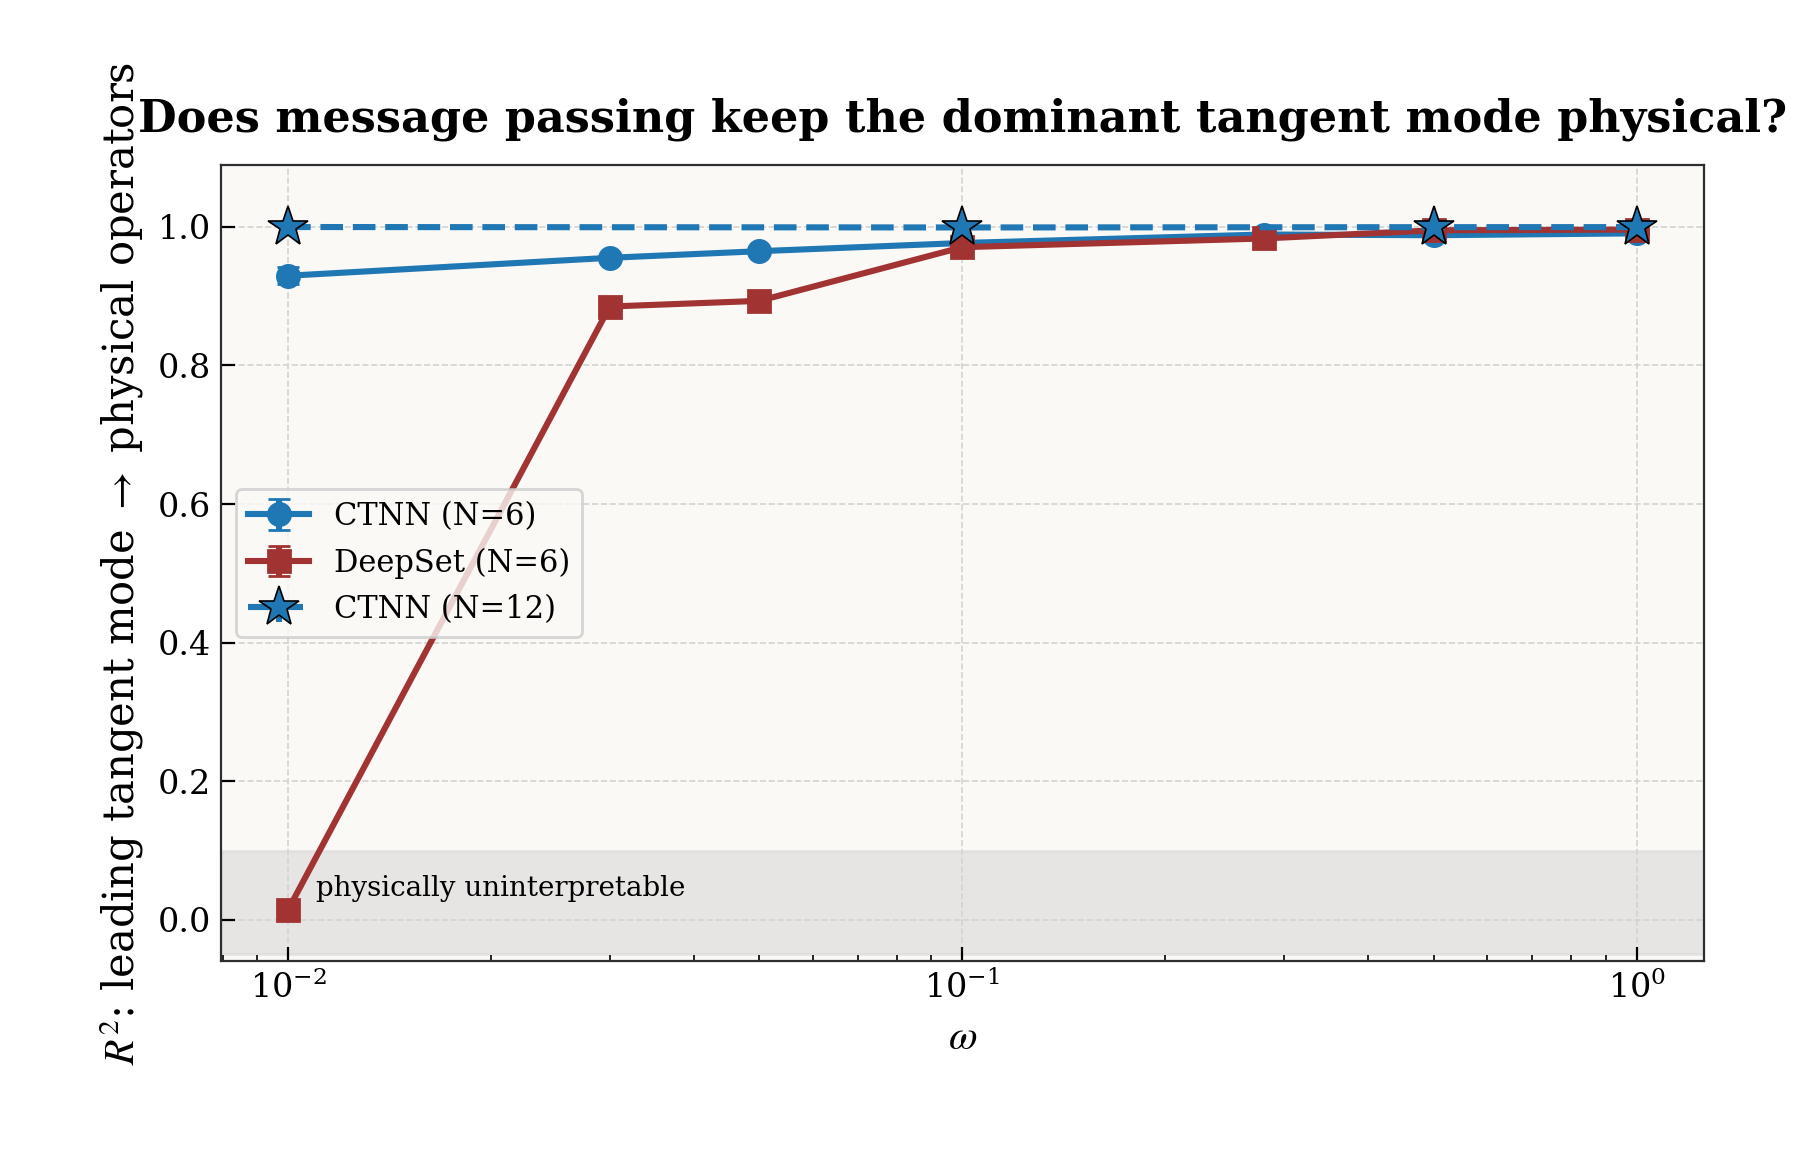
\includegraphics[width=0.9\textwidth]{mode_naming_scan.png}
  \caption[Leading-mode fit to the selected operator dictionary]{$R^2$ of the correlator's
  leading tangent-kernel eigenmode against the selected four-operator dictionary,
  seed-averaged over well-trained checkpoints. The CTNN retains a high dictionary fit across
  the grid; the DeepSet fit falls at weak confinement. No random-dictionary null or held-out
  fit was run, so this is a relative comparison. Three seeds at $\omega=0.01$.}
  \label{fig:mode-naming}
\end{figure}

\paragraph{The dominant mode is not the tangent space.} Figure~\ref{fig:mode-naming} scores
the \emph{dominant} eigenmode against the dictionary; Fig.~\ref{fig:nonphys} asks where the
eigenvalue-weighted mass of the leading modes \emph{as a whole} lies. A network can place its
largest mode squarely inside the dictionary and spend most of the rest outside it, which is
what the separable network does---so the leading-mode score is generous to it. At $\omega=1$
it has the slightly higher leading-mode fit ($R^2\approx0.996$ against $0.991$), with
energies identical to four figures. Write the
eigenvalue-weighted fraction of the top tangent modes lying \emph{outside} the
selected-operator span as the \emph{dictionary-orthogonal tangent mass}. The DeepSet carries a large
excess at \emph{every} confinement---$0.44$ against the CTNN's $0.06$ at $\omega=1$, a gap of
$\sim\!0.3$--$0.5$ that persists from the strongly-confined limit down to the crystal
(Fig.~\ref{fig:nonphys}). Thus the separable network can reach the same energy while leaving
nearly half its tangent weight along directions the selected dictionary does not resolve.
Those directions are not necessarily unphysical; the result is only that these four
operators account for one tangent space more completely than the other. Nor is this merely a
consequence of the CTNN's smaller $d_{\mathrm{eff}}$: toward the Wigner regime the two
effective dimensions converge to ${\sim}3.7$ while the dictionary gap persists. At $N=12$
the contrast is stronger still: the CTNN's dictionary-orthogonal mass stays
$\lesssim\!0.02$ across $\omega$, while a matched DeepSet trained to $+0.2\%$ sits at
$\approx\!0.77$ at $\omega=1$.

\begin{figure}[htbp]\centering
  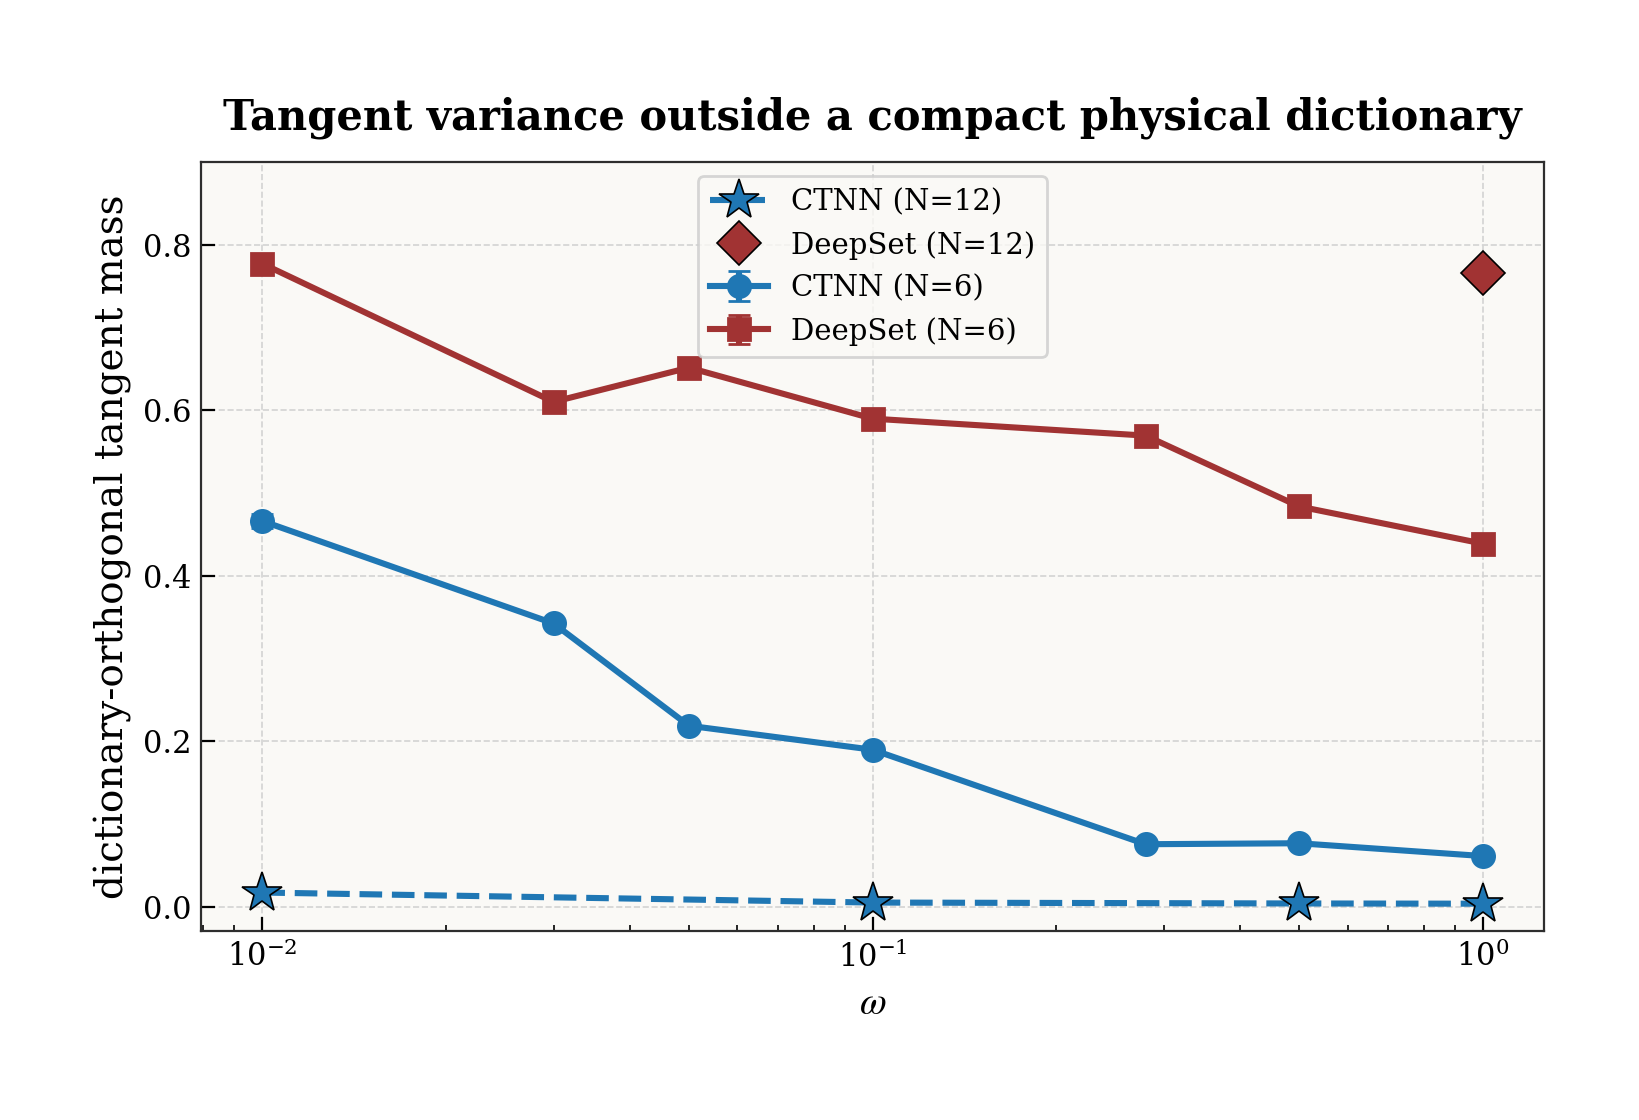
\includegraphics[width=0.85\textwidth]{nonphys_mass.png}
  \caption[Dictionary-orthogonal tangent mass against $\omega$]{Dictionary-orthogonal
  tangent mass---the eigenvalue-weighted tangent variance outside the span of the selected
  four-operator dictionary---against
  $\omega$. At $\omega=1$, where the two correlators agree in energy to $0.001\%$, the DeepSet
  places $44\%$ of its tangent variance outside the dictionary and the CTNN $6\%$; the excess
  persists at every $\omega$.}
  \label{fig:nonphys}
\end{figure}

\subsection{The backflow: rank collapse and its absence}
\label{sec:kernel-q1b}

The contrast is sharper in the backflow, but the comparison is less controlled. The
correlator, data, training protocol and optimiser are shared; capacity, coordinate
preprocessing and centre-of-mass projection are not (\S\ref{sec:bf-init}). At the production
width the copresheaf network has $182$k parameters and the conventional network $51$k, and
no matched pair was trained. The results therefore compare the archived implementations,
not message routing alone.

At $\omega=1$ both implementations reach reference quality, but they diverge as the trap
weakens (Table~\ref{tab:bf_energies}). The CTNN backflow stays within $0.01$--$0.12\%$ across
all $N$ and $\omega$, whereas the conventional backflow reaches $+0.58\%$ at
$N=6,\omega=0.01$ and $+0.69\%$ at $N=20,\omega=0.01$, about six times the CTNN error there.

\begin{table}[htbp]\centering
\caption{Relative energy error (\%) of the two backflow architectures, seed-averaged.}
\label{tab:bf_energies}
\begin{tabular}{l|cc|cc|cc}
\hline
 & \multicolumn{2}{c|}{$N=6$} & \multicolumn{2}{c|}{$N=12$} & \multicolumn{2}{c}{$N=20$}\\
$\omega$ & CTNN & conv & CTNN & conv & CTNN & conv \\
\hline
1.0  & $-0.03$ & $+0.06$ & $-0.01$ & $+0.04$ & $+0.06$ & $+0.07$ \\
0.1  & $-0.05$ & $+0.16$ & $+0.01$ & $+0.16$ & $+0.02$ & $+0.18$ \\
0.01 & $-0.04$ & $+0.58$ & $-0.01$ & $+0.54$ & $+0.12$ & $+0.69$ \\
\hline
\end{tabular}
\end{table}

\paragraph{How component-level numbers are read.}
\label{sec:synthesis}
Energy and $\Var(E_L)$ are state-level quantities; the backflow's rank, displacement
magnitude and component-wise $d_{\mathrm{eff}}$ are not. Because the correlator and backflow
can substitute for one another, these component-level diagnostics record the training route
as well as the state it reached.

This distinction matters here. An earlier rank collapse under joint, from-scratch training
affected both architectures, moved with the seed and carried no energy penalty. The collapse
reported below occurs under the staged protocol, affects only the conventional backflow, is
seed-robust where replicated and accompanies an energy loss. The energetic change makes it
more than a component-level curiosity.

We define the \emph{backflow rank} as the participation ratio of the displacement field
$\Delta\mathbf{x}$: the effective number of independent directions along which the backflow
moves the electrons.

The columns of Table~\ref{tab:bf_rank} have different ceilings: $2N-2$ for the copresheaf
network, which projects out the mean displacement, and $2N$ for the conventional network.
Their absolute levels are therefore not directly comparable. The change with confinement is.
At $\omega\ge0.1$ the conventional field remains near its ceiling; at $\omega=0.01$ it
collapses to rank~$1$ for $N=6$, $12$ and $20$, while the CTNN field remains near full rank.
The tangent dimension changes in the same direction, growing from ${\sim}4$ to ${\sim}10$
for the CTNN and falling from ${\sim}6$ to ${\sim}1$ for the conventional backflow. The
rank-one result is reproduced by both seeds at $N=6$ and $N=12$; the $N=20$ value is from a
single re-run. Because the conventional field retains a centre-of-mass component, the
rank-one endpoint cannot yet be identified with a relative collective mode.

\paragraph{What the comparison supports.} The core observation is simple: in the Wigner
regime the conventional implementation collapses to a rank-one displacement field and its
energy degrades, whereas the CTNN implementation does neither. The cause is not isolated.
The conventional network is a third the size, only the CTNN scales its inputs by
$\sqrt{\omega}$, and only the CTNN removes the mean displacement. The same conventional
network works above the Wigner regime, so the failure is confinement-dependent, but that
does not distinguish capacity, preprocessing and architecture.
Tables~\ref{tab:bf_energies} and~\ref{tab:bf_rank} therefore describe the production
implementations used in Chapter~\ref{ch:results}; they are not an architecture ablation.

\begin{table}[htbp]\centering
\caption[Backflow displacement rank (participation ratio)]{Backflow displacement rank
(participation ratio), evaluated on the field returned by each network. The ceilings are
$2N-2$ ($10/22/38$) for the copresheaf network and $2N$ ($12/24/40$) for the conventional
one, so compare the collapse rather than the absolute levels. The networks are not
capacity-matched ($182$k against $51$k). Entries are two-seed means except at $N=20$,
$\omega=0.01$, which is a single re-run whose per-run rank artefacts were not retained.}
\label{tab:bf_rank}
\begin{tabular}{l|cc|cc|cc}
\hline
 & \multicolumn{2}{c|}{$N=6$} & \multicolumn{2}{c|}{$N=12$} & \multicolumn{2}{c}{$N=20$}\\
$\omega$ & CTNN & conv & CTNN & conv & CTNN & conv \\
\hline
1.0  & $8.8$ & $10.4$ & $20.8$ & $22.2$ & $36.9$ & $35.4$ \\
0.1  & $7.7$ & $10.4$ & $18.2$ & $21.7$ & $33.8$ & $37.6$ \\
0.01 & $9.8$ & $\mathbf{1.0}$ & $20.8$ & $\mathbf{1.0}$ & $35.2$ & $\mathbf{1.0}$ \\
\hline
\end{tabular}
\end{table}

\paragraph{Pricing each component by deletion.} We next ablate components on a common probe
drawn from the full model's $|\Psi|^2$. Holding the configurations fixed isolates the change
in the kinetic term when a component is removed. It does not give the energy of a relaxed
ablated state, so these numbers rank local contributions rather than energetic costs.

(i) On this probe the \textbf{backflow's share shrinks and the Jastrow messages' share grows}
as the trap weakens. Deleting the backflow costs $+5.6\%$ at $\omega=1$ and $+1.4\%$ at
$\omega=0.1$, but only $+0.013$--$0.017\%$ at $\omega=0.01$ (three seeds), while deleting the
Jastrow messages runs the other way: $+3.9\%$ at $\omega=1$ rising to $+9$--$15\%$ at
$\omega=0.01$. A variational deletion on separately sampled production-width networks gives
the opposite trend: removing the message-passing backflow costs $0.5\%$ at $\omega=1$,
$1.0$--$1.2\%$ at $\omega=0.1$ and $1.9$--$2.0\%$ at $\omega=0.01$. The methods and networks
differ, and the division of correlation between components is route-dependent, so neither
result establishes a physical migration of relational work from nodes to amplitude. The
conclusion that survives is:

(ii) \textbf{Within the backflow, the transport maps \emph{are} the displacement}: zeroing
the inter-particle transport maps ($\rho_{v\to e},\rho_{e\to v}$) perturbs
$\Delta\mathbf{x}$ by as much as deleting it outright---the mean
$|\Delta\mathbf{x}_{\mathrm{abl}}-\Delta\mathbf{x}|$ is comparable to the mean
$|\Delta\mathbf{x}|$ at every $(N,\omega)$. The displacement therefore comes primarily from
the transported messages, not the per-particle path. Both architectures use relative
coordinates, but the conventional backflow aggregates one round of pairwise messages per
particle, whereas the CTNN maintains an explicit edge state across the graph. Empirically,
the former does not sustain a high-rank displacement field at the crystal; the latter
does, and its transport maps carry almost the entire displacement.

\begin{figure}[htbp]\centering
  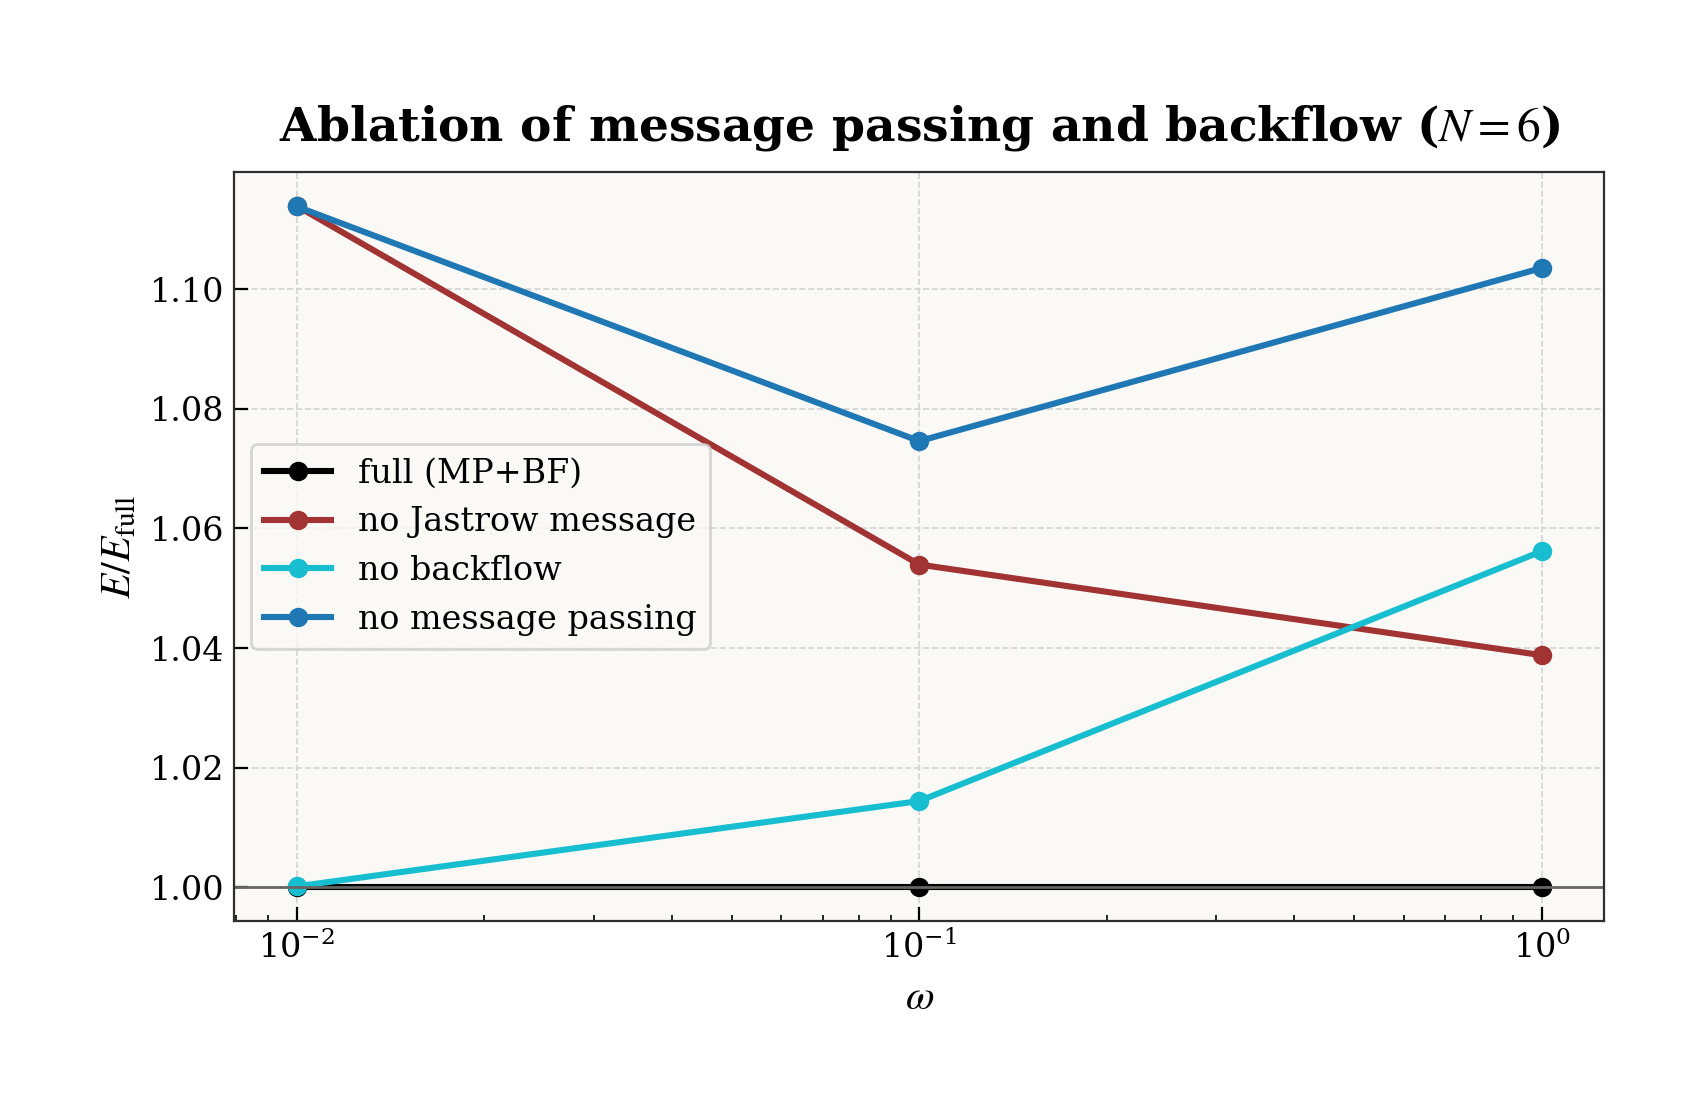
\includegraphics[width=0.85\textwidth]{message_ablation.png}
  \caption[Fixed-measure ablation cost of each component]{The \emph{fixed-measure
  instantaneous ablation cost} of each component (trained networks, $N{=}6$). Configurations
  are drawn once from the full model's $|\Psi|^2$ and every arm is re-evaluated on them, so
  $\Delta E_{\rm probe}/E_{\rm full}$ is the change in the kinetic term when a component is
  switched off, not the energy of a retrained network. Cyan: backflow removed; dark red:
  Jastrow messages removed; blue: all message passing removed. The curves cross near
  $\omega\approx0.4$. The trend reverses when the ablated production-width networks are
  evaluated variationally on their own samples (text).}
  \label{fig:q1b-ablation}
\end{figure}

\subsection{Evidence consistent with a common relational bottleneck}
The two effects may share a cause in how relational information is routed. The separable
correlator pools independently encoded pairs, and the conventional backflow aggregates one
round of pairwise messages; neither retains a transported edge state. The CTNN variants do.
To test whether the two diagnostics move together, we retained the conventional backflow in
both arms, changed the correlator family, retrained each arm and followed the sweep in
$\omega$.

The backflow's failure boundary moves with the correlator. With a separable correlator the
two give way together near $\omega\approx0.05$: correlation-hole capture falls from $0.68$
to $0.07$ and the displacement rank from ${\sim}10$ to $1$ across the same step. With a
message-passing correlator both hold half a decade further, to $\omega\approx0.01$
(Fig.~\ref{fig:q1-unify}).

Each arm is a separately trained model, and the correlators differ in primitive features as
well as routing. The co-movement is therefore consistent with a shared relational bottleneck,
but does not exclude feature scaling, optimisation path or capacity as common causes.

\begin{figure}[htbp]\centering
  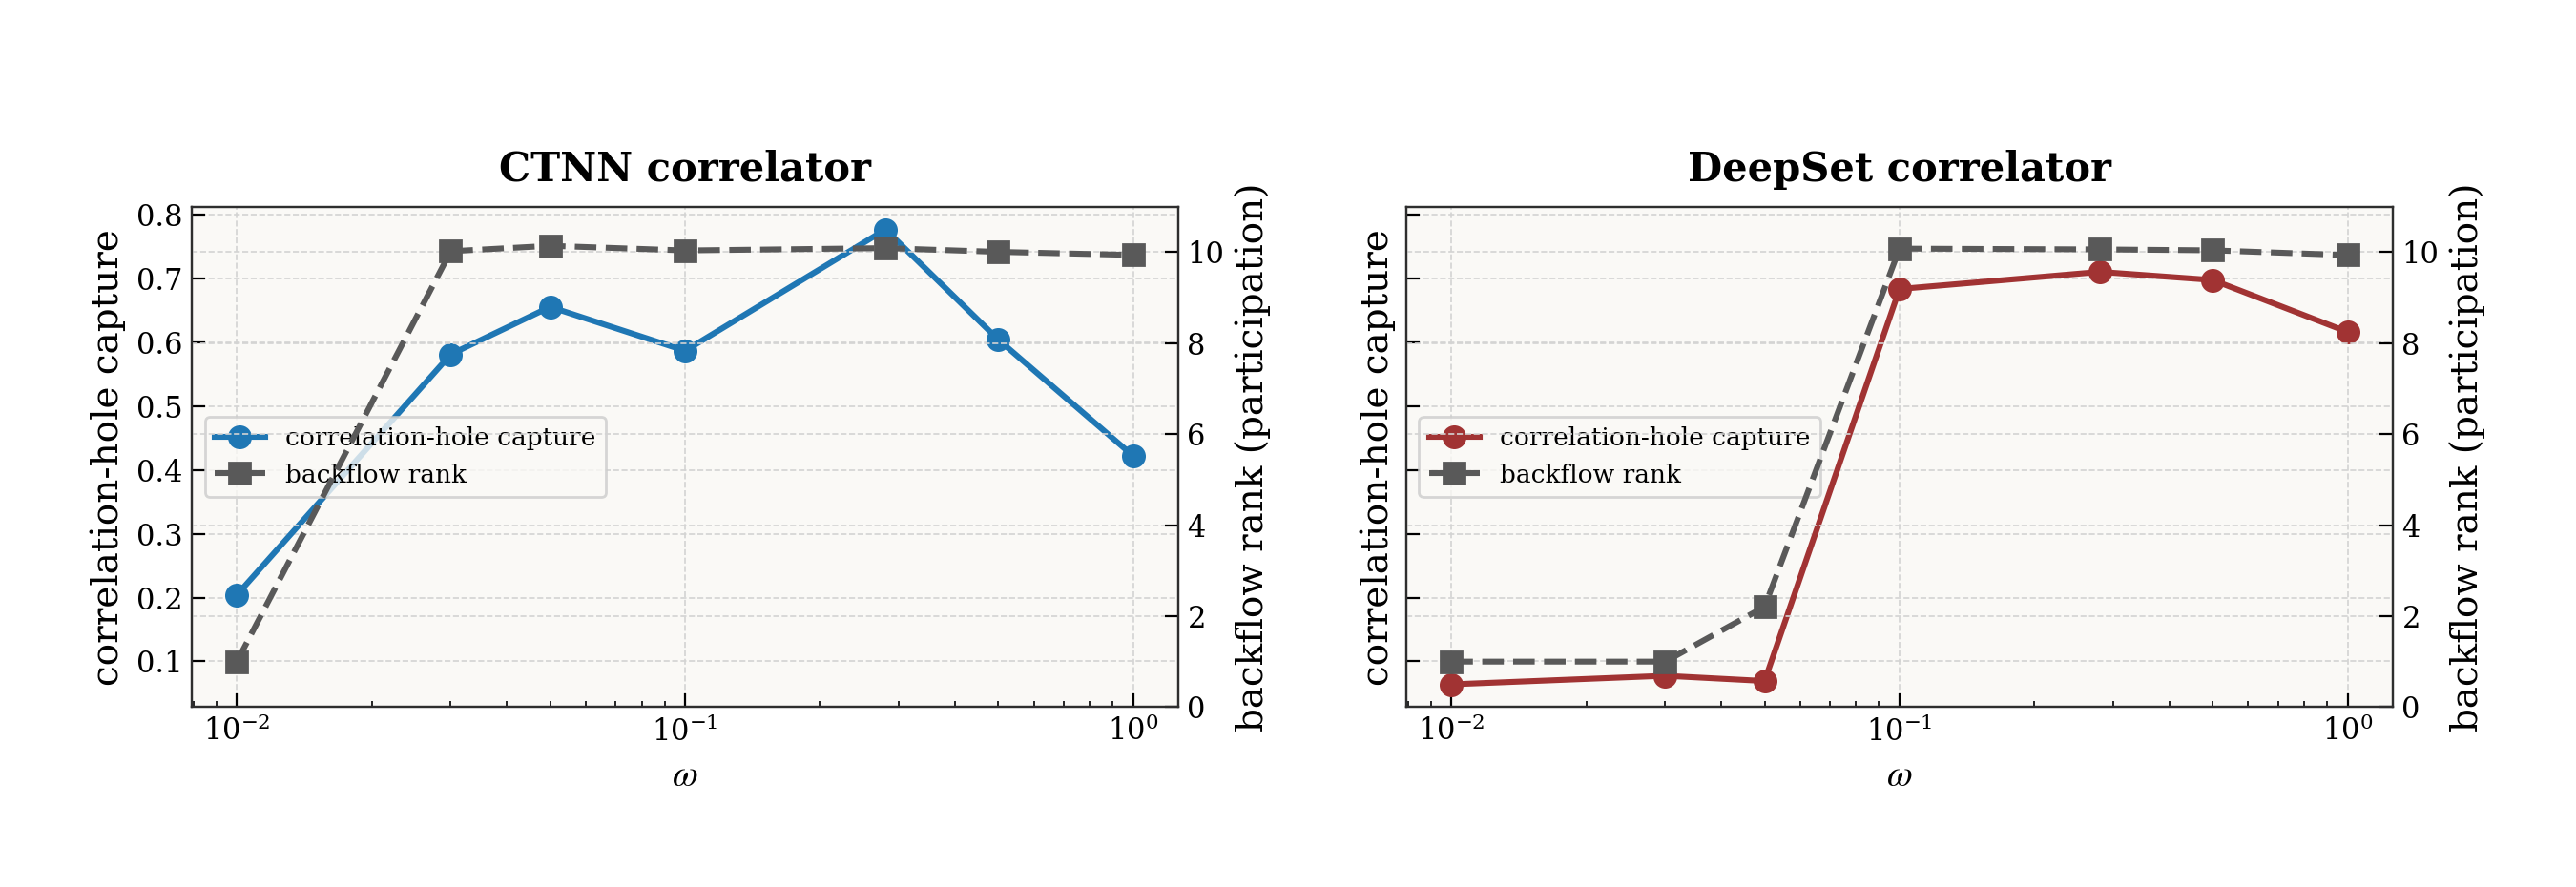
\includegraphics[width=\textwidth]{q1_unification.png}
  \caption[Correlator dictionary fit and backflow rank across confinement]{Correlator
  dictionary fit and backflow displacement rank for $N=6$, with the conventional backflow
  used in both arms. For each correlator family, the
  correlation-hole capture (left axis) and the backflow displacement rank (right axis) give way
  at the same $\omega$: $\omega\!\approx\!0.05$ for the DeepSet, $\omega\!\approx\!0.01$ for the
  CTNN. The co-movement is consistent with a shared bottleneck, but the correlator features
  are not otherwise matched.}
  \label{fig:q1-unify}
\end{figure}
\FloatBarrier

% =====================================================================
\subsection{What the trained representation looks like}
\label{sec:kernel-repr}

One descriptive result belongs beside these controlled comparisons. Examining a single
high-quality trained solution shows the correlator occupying a feature space of one to three
effective dimensions across the entire grid and never expanding: at $\omega=10^{-3}$, where
the real-space density has developed rings and discrete occupancies, the latent rank is no
larger than at $\omega=1$. What changes across the crossover is which branch the leading axis
draws on, not how many axes there are. The displacement field is the opposite kind of object,
spanning nearly all the spatial directions available to it and leaving the correlator's
feature geometry almost unperturbed.

These are component-level measurements on one run. They are gauge-like---the correlator and
backflow are partial substitutes, so the division of labour between them records the training
route as much as the state---and no architectural conclusion above depends on them. They are
recorded because a low effective covariance rank is not what one would predict for a
state whose real-space structure is this elaborate, and because the reorganisation happens
near $\omega\approx0.1$, the same confinement at which the energy partition crosses over
(\S\ref{sec:wigner-energy}). Whether that coincidence reflects one mechanism or two we cannot
say from a single run. Appendix~\ref{app:representation} gives the full analysis.

\medskip
\noindent The implemented correlator families differ before their energies do. Under the
parametrisations used here, the CTNN concentrates its Fisher weight in fewer directions at
strong confinement and is better described by the selected dictionary; its local-energy
variance is also lower by factors of $1.2$ to $3.4$. In the backflow sweep, the conventional
implementation collapses to rank one and loses half a percent where the CTNN does not. Since
the comparisons are not matched in every feature, scale and constraint, these are findings
about the archived implementations rather than message passing alone; their co-movement
motivates the shared-bottleneck hypothesis. The state-level result is the variance:
correlators that agree in energy to four figures but differ in variance have reached
different \emph{states}. Their overlap was not measured, so the variance does not quantify
that difference.

\section{Conditioning and the sampling measure}
\label{sec:kernel-cond}
\label{sec:kernel-q2}

Two design choices remain, and the tangent geometry connects them. One asks what a
natural-gradient step buys over a diagonal one. The other asks what changes when the loss is
defined by an analytic proposal instead of by $|\Psi|^2$. They are the same question twice
over: stochastic reconfiguration inverts the metric $S$, and the sampling measure is what
builds $S$ in the first place.

\subsection{Natural-gradient preconditioning}
Stochastic reconfiguration preconditions the gradient by the inverse QGT,
$\btheta \leftarrow \btheta - \eta\, S^{-1}\nabla_{\btheta} E$; geometrically it \emph{whitens} the tangent
kernel. At $N=2$ this is exact: the SR step aligns with the imaginary-time direction
to numerical precision. The question is where whitening changes the outcome.

Fixing the ansatz and varying only the optimiser from a common stage-3 base:
\textbf{for $|\Psi|^2$-VMC, SR and Adam are indistinguishable}---exact at $N=2$
(var $\sim\!10^{-9}$), and at $N=6$ the energy gap
$E_{\mathrm{Adam}}-E_{\mathrm{SR}}$ is $\lesssim0.002$ across $\omega$ and both
seeds; in the matched pair at $\omega=1$ the two agree to four decimals in relative error.
\textbf{For weak-form collocation from the same common base, SR is decisive}: there
$E_{\mathrm{Adam}}-E_{\mathrm{SR}}$ is large and positive (e.g.\ $+2.9$ at
$N=6,\omega=1$), and plain Adam does not converge the objective.

This controlled comparison does not conflict with \S\ref{sec:colloc-method}, where Adam is
the production default. With a bare objective and fixed proposal, the collocation gradient
stalls under a diagonal step and SR rescues it. The production pipeline instead controls the
gradient at its source through proposal refitting, oversampling, reward normalisation,
rollback and cascade warm-starting; once these are in place, Adam suffices, although their
individual effects were not isolated (\S\ref{sec:gradient-chain}). Below
$\omega\simeq0.01$, the samples used to build $S$ collapse and SR becomes unstable, so Adam
is the more robust default. Its large speed advantage in our code mainly reflects the
per-sample loop used to construct the score matrix: vectorising that calculation makes it
$25$ times faster at $N=6$ and $82$ times faster at $N=20$
(Appendix~\ref{app:walltime}). The comparison here concerns what SR buys, not what it costs.

A large condition number alone does not explain the difference. Table~\ref{tab:kappa}
reports
$\kappa(S)=\lambda_{\max}/\lambda_{\min}$ measured on the trained states under $|\Psi|^2$
sampling, and it is enormous, $10^{7}$ to $10^{10}$, for \emph{both} architectures and at
every capacity in the ladder, including precisely the models on which Adam and SR agree to
four decimals. Whatever makes SR unnecessary under $|\Psi|^2$ sampling, it is not that the
metric is well conditioned.

\begin{table}[htbp]\centering
\caption[Condition number of the empirical geometric tensor]{Condition number of the
empirical quantum geometric tensor at $N{=}6$, $\omega=1$, measured on each trained state's
own $|\Psi|^2$ samples at fixed batch $B=768$. Since $B<P$, $\lambda_{\min}$ is the smallest
sample-supported eigenvalue and depends on batch size, regularisation and the numerical
threshold; $\kappa$ should therefore be read by order of magnitude. The
$d_{\mathrm{eff}}$ values use the same finite batch rather than the converged common probe of
\S\ref{sec:kernel-q1a}, and are included only to show that $\kappa$ does not track them. Adam
and SR reach the same energy on every row.}
\label{tab:kappa}
\begin{tabular}{llcc}
\hline
architecture & params & $\kappa(S)$ & $d_{\mathrm{eff}}$ \\
\hline
CTNN (seed 1)      & $79.8$k & $6.9\times10^{7}$  & $1.46$ \\
CTNN (seed 2)      & $79.8$k & $5.2\times10^{7}$  & $1.39$ \\
DeepSet (small)    & $20.2$k & $3.2\times10^{9}$  & $3.56$ \\
DeepSet (medium)   & $47.7$k & $3.4\times10^{7}$  & $4.35$ \\
DeepSet (matched)  & $89.4$k & $3.2\times10^{10}$ & $3.61$ \\
DeepSet (large)    & $164$k  & $1.4\times10^{7}$  & $4.76$ \\
\hline
\end{tabular}
\end{table}

For the tested $N=2$ and $N=6$ cases, the data rule out condition number alone. Our working
hypothesis is that SR matters when the tangent metric is anisotropic and still statistically
estimable; a noisy or rank-deficient estimate can make $S^{-1}$ amplify rather than suppress
noise. The instability of CG-SR at ultra-weak confinement is consistent with this account
(\S\ref{sec:colloc-negatives}). The criterion remains a hypothesis because the
collocation-space spectrum was not measured at matched batch size; neither the optimiser
comparison nor the spectrum measurement was extended to $N=12$ or $20$.

% =====================================================================
\subsection{Consequences of the sampling measure}

VMC and importance-sampled collocation use the same Slater--Jastrow--backflow form, but the
reported models are not capacity matched. Their training also changes the loss and its
sampling measure. The following three consequences concern that measure change; they are
not controlled architecture comparisons.
\paragraph{Target sampling aligns the estimator with the metric; a covering proposal does
not.} Sampling from $|\Psi|^2$ makes the estimators of $S$ and of the gradient share the
measure that defines them, so the directions carrying Fisher weight are also the directions
the batch populates. That is an alignment between estimator and objective, not
preconditioning in the sense of applying $S^{-1}$. A fixed covering proposal instead drives
a monotone \emph{ESS collapse} as $N$ and $1/\omega$ grow: at $N=6,\omega=0.01$ the
effective sample size, measured against a converged state, falls to $0.11\%$ of the
batch---about $5$ of the $4096$ retained points---and the gradient estimator is then
degenerate. (Table~\ref{tab:ring-ess} finds $1.5$ for the same mixture against a different
converged checkpoint at the same $(N,\omega)$; at a handful of effective points the ESS is
itself a noisy number, and the two are the same collapse.) In this setting the result
diagnoses severe estimator failure; continued training with the same static proposal does
not address the lost overlap. (Two ESS normalisations appear in this chapter, differing by
the oversampling factor; each figure states which.)

\S\ref{sec:colloc-reliability} below nonetheless reports usable collocation energies at the
same $(N,\omega)$---$+0.22$--$0.26\%$ across three seeds, Table~\ref{tab:reliability}---and
the two situations differ in the sampler and in the quantity being described. The sampler
first: the collapse measured above is for the \emph{static} origin-centred
mixture, while the campaign's robust recipe refits its proposal every $30$ epochs and
oversamples $16\times$. The campaign's \emph{baseline} rows, which keep the static
proposal, are the ones that blow up ($+3.9$ to $+7.2\%$ at $\omega=0.001$). Second, and
more interesting, the two statements are not about the same quantity. The energy stays within a third of a percent while the modulus overlap ceases to be
resolvable---which is the sharpest illustration in this thesis of why energy alone does not
certify a state. We stop short of saying the overlap \emph{is} zero: $\mathcal{S}^2$ is a
ratio estimator built from the same degenerate weights, so at this ESS it reports \emph{unresolved} and not orthogonal.

\begin{figure}[htbp]\centering
  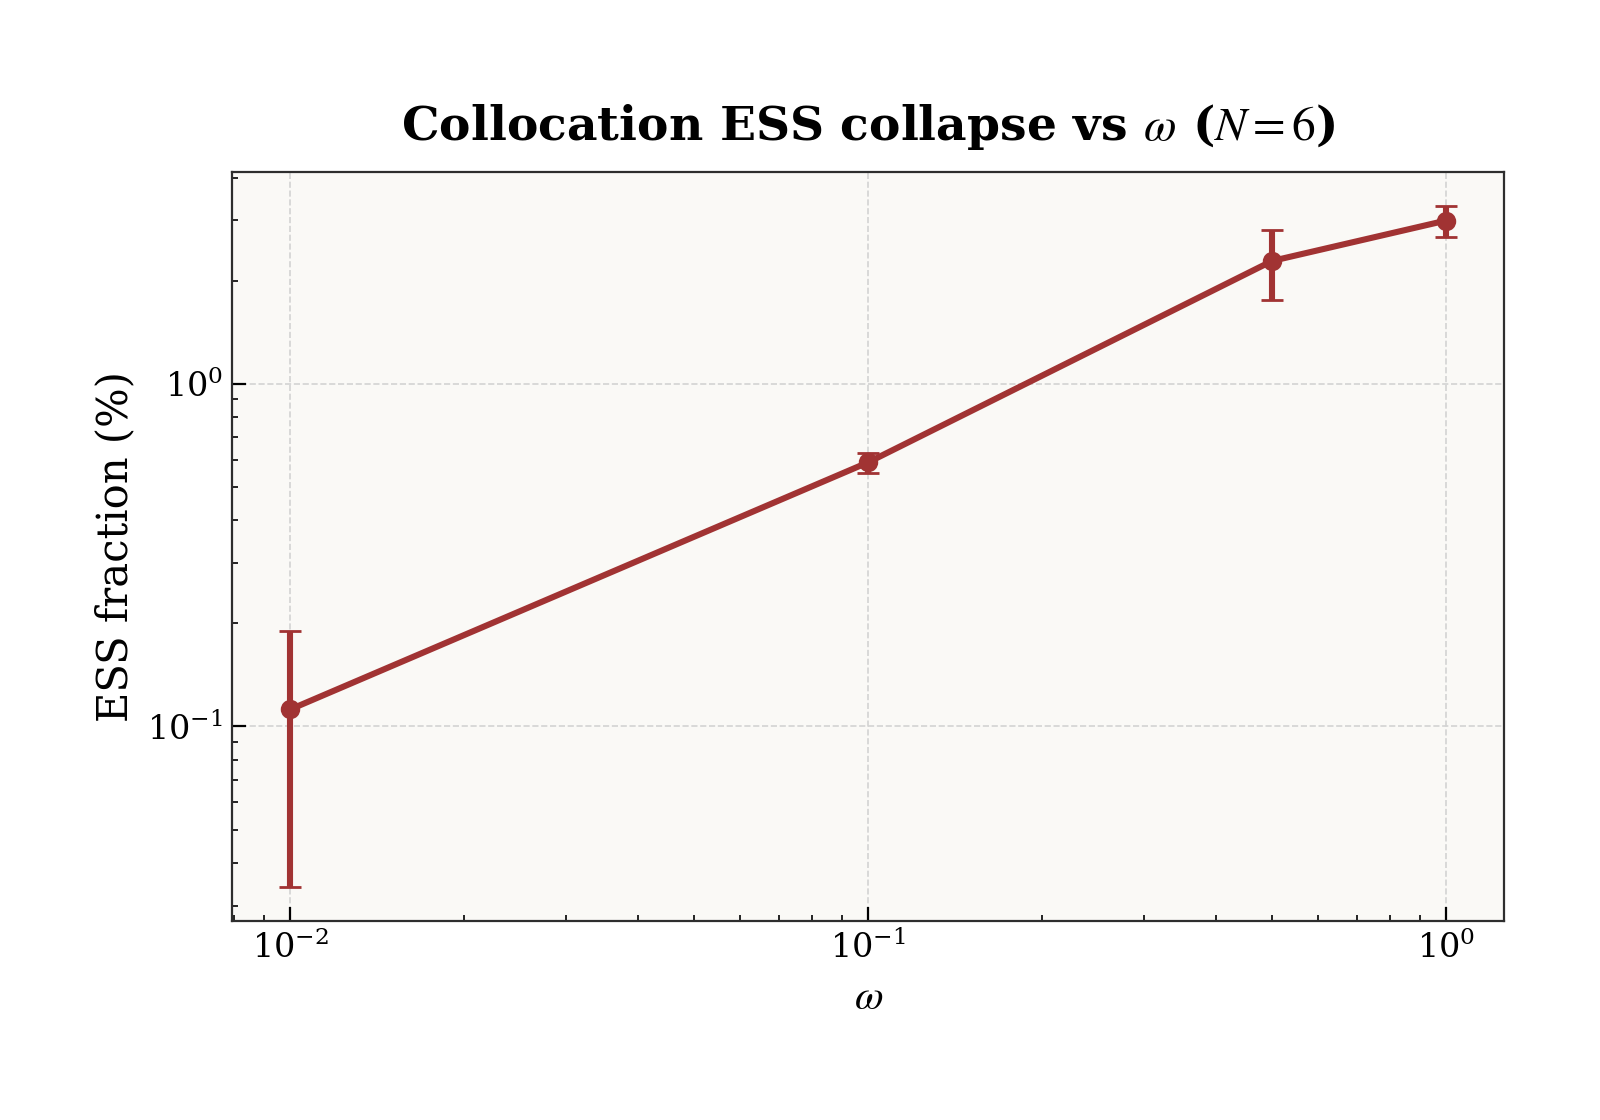
\includegraphics[width=0.8\textwidth]{ess_collapse.png}
  \caption[ESS collapse of the naive collocation proposal]{The naive collocation proposal collapses in the Wigner regime ($N{=}6$). The
  effective sample size (as a percentage of the batch) falls by more than an order of
  magnitude from $\omega{=}1$ to $\omega{=}0.01$, where it reaches $\sim\!0.1\%$---about five
  usable points in a batch of $4096$. This diagnoses proposal--target mismatch for the
  sampled state and motivates the physics-informed ring proposal of
  \S\ref{sec:kernel-q3-frontier}, which is designed to repair it.}
  \label{fig:q3-ess}
\end{figure}

\paragraph{Amplitude agreement degrades with proposal overlap.} We test whether the two
paradigms reach similar wavefunction amplitudes, rather than merely similar energies, using
the symmetric modulus-overlap diagnostic
$\mathcal{S}^2=\langle\Psi_B/\Psi_A\rangle_{|\Psi_A|^2}
\langle\Psi_A/\Psi_B\rangle_{|\Psi_B|^2}$. At $N=2$ the amplitudes agree closely
($\mathcal{S}^2>0.997$ for every $\omega$, both optimisers, both seeds): the paradigm
is efficiency-only, collocation paying $\sim\!5\times$ the variance for essentially the
same amplitude. At $N=6$ they \emph{diverge}: under Adam $\mathcal{S}^2$ falls from $0.85$ at $\omega=1$ to
$0.77$ at $\omega=0.1$ (both seeds), tracking the ESS collapse, and at $\omega=0.01$ the
estimator returns values near zero but is no longer resolved---at an ESS of about five
points it is a ratio of two degenerate importance-weighted averages, and we record it as
\emph{unresolved} rather than as a measured orthogonality. SR partially rescues the
$\omega=0.1$ value ($\mathcal{S}^2\!\approx\!0.95$) but does not close the gap. Weak-form
collocation reaches essentially the same amplitude as VMC at the two-electron anchor. At $N=6$
the amplitudes already differ at strong confinement and become harder to compare as proposal
overlap deteriorates.
In these tests, the route that benefits from SR is also the one that becomes unreliable as
the proposal loses overlap. An adaptive proposal that tracks $|\Psi|^2$ is the next remedy tested in
\S\ref{sec:kernel-q3-frontier}.

\paragraph{Why the collocation energy readout is biased.} For an exact eigenstate the
local energy $E_L=\hat H\Psi/\Psi$ is constant over configuration space, so
$\Var(E_L)\to0$ as the ansatz approaches the ground state---the zero-variance principle,
and the reason $\Var(E_L)$ is a sharp quality measure. That cancellation is a property of
the \emph{full} local energy, in which the kinetic (Laplacian) and potential terms combine
to a constant; it is not a property of the Laplacian term alone. The collocation objective
does \emph{not} discard the Laplacian: it is a score-function (REINFORCE) estimator that
\emph{forms} the full $E_L$ as a detached reward and differentiates only $\log|\Psi|$
(\S\ref{sec:colloc-method}). What it gives up is the \emph{measure}, and three things then spoil the readout, in
increasing order of severity. The estimator is self-normalised, since $|\Psi_\theta|^2$ is
unnormalised, so it carries an $\mathcal O(1/n)$ finite-sample bias that vanishes with sample
size. The tail controls deliberately change the target: tempering $w\to w^\alpha$ and
clipping the log-weights trade bias for variance on purpose, so the estimated quantity is no
longer $\langle E_L\rangle_{|\Psi|^2}$. And, dominant in the regimes that matter,
proposal--target mismatch inflates the variance beyond any affordable sample size
(\S\ref{sec:colloc-reliability}). Importance sampling is not biased merely for being
importance sampling; it is the last two that make the readout unusable as a stopping rule.
The reliable readouts are $\Var(E_L)$ and the modulus overlap, both on $|\Psi|^2$ samples, and
for the same reason no energy reported in this thesis is an importance-sampling estimate:
every one is a Metropolis evaluation of $|\Psi|^2$.

The practical question is therefore how far an analytic proposal can preserve usable
gradient statistics without a Markov chain.

\section{Training with MCMC-free gradient updates}
\label{sec:kernel-mcmcfree}
\label{sec:collocation}

The conditioning story has a practical edge. If the sampling measure is what makes the
metric estimable, then choosing that measure is a design decision, not a fact of nature---and
the obvious thing to try is a measure with no Markov chain in it at all. ``MCMC-free''
refers to the gradient throughout: no configuration entering a parameter update comes from a
chain, but a Metropolis probe still selects checkpoints and certifies the final energy, and
the cascades start from reference-guided pretrained states
(\S\ref{sec:collocation-discussion} states the claim exactly).

\paragraph{Two distinct limits.}
The method encounters proposal degeneracy and failure to transfer a checkpoint between
confinements. The results below separate them.

\emph{The first limit is statistical.} A fixed analytic proposal loses overlap with
$|\Psi_\theta|^2$ as the trap opens; the importance weights grow heavy-tailed; the gradient
estimator comes to be dominated by a handful of draws; the empirical metric becomes
unreliable and preconditioning can then amplify noise. The evidence is consistent with a
sampling limit, and a better proposal moves the observed boundary---from $\omega\approx0.01$ with an
origin-centred mixture to $\omega=0.0035$ with one built out of the measured Wigner
geometry.

\emph{The second limit concerns transfer.} Below $\omega=0.0035$ a stable trained state fails
to survive transfer to a weaker trap even when the sampler is initialised directly on the
correct shell. Diagnostics point to a near-balance between the confining determinant and
the compensating Jastrow, which is disturbed by the $23\%$ change in $\omega$. Correct
shell initialisation alone does not repair the transferred state.
It limits the cascade, which carries trained states down in small steps of $\omega$,
and not for MCMC-free gradient updates as such: started instead from a pretrained checkpoint,
the reliability campaign of \S\ref{sec:colloc-reliability} trains $N{=}6$ at $\omega=10^{-3}$
to within $0.35\%$ of our SR--VMC energy.

\noindent \S\ref{sec:kernel-mcmcfree} documents the proposal-degeneracy evidence;
\S\ref{sec:kernel-q3-frontier} moves that observed boundary and then encounters the transfer
failure.

A Markov chain is what makes neural variational Monte Carlo sequential. Chains must
equilibrate, successive samples are correlated, and mixing times grow with particle number
and with correlation strength. They grow fastest, in other words, exactly where the physics
gets interesting.

Draw the configurations instead from a fixed analytic proposal and reweight them, and the
whole gradient step becomes embarrassingly parallel. The question is what that costs.

Two ways of posing the problem behave very differently, and the difference decides
everything downstream. The \emph{strong form} asks the wavefunction to satisfy the local
Schr\"odinger equation pointwise, minimising the variance of $E_L$ and differentiating
through the Laplacian to do it. The \emph{weak form} uses a score-function (REINFORCE)
gradient in which the Laplacian enters only as a reward and is never differentiated.
Appendix~\ref{app:catch22} shows why this is difficult for a backflow: $E_L$ generally has a
pole at a simple trial node, and differentiating through a node that moves with the
parameters makes the empirical gradient more singular. None of the tested combinations of
sampling, loss and preconditioning improved beyond an error near $0.3\%$. Model sizes were
not matched to production VMC, so the experiment motivates the change of objective without
identifying the objective as the sole cause. Everything below uses the weak form.

Using the same Slater--Jastrow--backflow ansatz form, and with no
Markov chain in any gradient, the weak form comes within about a tenth of a percent of DMC
at strong confinement and within about a third of a percent of our lowest SR--VMC energies
well into the correlated regime for $N\in\{6,12\}$ (Table~\ref{tab:collocation}). The energies are collected here, where the method that
produced them is explained, rather than beside the SR--VMC energies of
\S\ref{sec:energy-overview}: without the failure mechanism of
\S\ref{sec:colloc-reliability} in hand, the pattern of where they hold and where they give
way is not interpretable.

\begin{table}[htbp]
  \centering
  \caption[Energies from MCMC-free gradient training]{Metropolis energies of
  states trained with MCMC-free gradients. Parentheses in the reported-energy column give
  standard errors. For $N{=}6$,
  both the best result and the mean $\pm$ standard deviation of three protocol-controlled
  seeds are shown. The $N{=}2$ and $N{=}12$ rows are single runs; $^{\dagger}$ marks
  continuation runs using the corrected proposal density. References are external where
  available and otherwise the lowest SR--VMC energy, so those deviations measure internal
  agreement. Energies are in effective Hartree.}
  \label{tab:collocation}
  \begin{tabular}{c c c c c c}
    \toprule
    & & & & \multicolumn{2}{c}{relative deviation (\%)} \\
    \cmidrule(lr){5-6}
    $N$ & $\omega$ & Reference & Reported energy & best & mean $\pm$ s.d. \\
    \midrule
    2 & 1.0   & $3.00000$      & $3.00105(44)$  & $+0.035$ & --- \\
      & 0.5   & $1.65977(1)$   & $1.65945(80)$  & $-0.019$ & --- \\
      & 0.1   & $0.44079(1)$   & $0.440944(56)$ & $+0.035$ & --- \\
      & 0.01  & $0.073839(2)$  & $0.073911(11)$ & $+0.098$ & --- \\
      & 0.001 & $0.013778$     & $0.013889(9)$  & $+0.806$ & --- \\
    \midrule
    6 & 1.0   & $20.15932(8)$  & $20.1731(18)$  & $+0.068$ & $+0.082\pm0.014$ \\
      & 0.5   & $11.78484(6)$  & $11.7952(12)$  & $+0.088$ & $+0.098\pm0.009$ \\
      & 0.1   & $3.55385(5)$   & $3.56393(24)$  & $+0.284$ & $+0.293\pm0.009$ \\
      & 0.01  & $0.69036$      & $0.691895(80)$ & $+0.222$ & $+0.244\pm0.020$ \\
      & 0.001 & $0.140832$     & $0.141175(4)$  & $+0.244$ & $+0.282\pm0.059$ \\
    \midrule
    12$^{\dagger}$ & 1.0 & $65.7001(1)$   & $65.7207(17)$  & $+0.031$ & --- \\
       & 0.5   & $39.1596(1)$   & $39.1727(12)$  & $+0.034$ & --- \\
       & 0.1   & $12.26984(8)$  & $12.28361(32)$ & $+0.112$ & --- \\
    \bottomrule
  \end{tabular}
\end{table}

\subsection{The weak-form objective}
\label{sec:colloc-method}
The collocation training used here is exactly the MCMC-free gradient pipeline specified in the
Methods: a weak-form (REINFORCE~\cite{Williams1992-REINFORCE}) objective in which the local energy
enters as a detached reward (\S\ref{sec:method-collocation},
Eq.~\eqref{eq:reinforce-method}), an analytic Gaussian-mixture proposal reweighted to
$|\Psi_\theta|^2$ with ESS / Pareto-$\hat k$ monitoring~\cite{Vehtari2024} and tail
controls (\S\ref{subsec:colloc-proposal}), and---in the Wigner
regime---the physics-informed ring proposal with cascade warm-starting
(\S\ref{subsec:colloc-wigner}). Two methodological findings shape what follows. First, among
the optimisers (\S\ref{sec:sr-stage}), \textbf{Adam} was the robust
default across all regimes, whereas \textbf{CG-SR} converged faster at $\omega\!\ge\!0.1$ but
diverged for $\omega\!\le\!0.01$, where the importance weights collapse. This is consistent
with an unresolved empirical metric, although that metric was not measured there directly.
Second, \textbf{cascade warm-starting}, initialising each confinement from a stable checkpoint at a stronger one, was decisive for reaching the deep-Wigner regime, exploiting
the transfer of correlation structure across $\omega$.


\label{sec:colloc-architectures}
Three ansatz families were tried within this framework. The Jastrow-only and backflow
variants share a Slater--Jastrow core; the neural Pfaffian changes the antisymmetric part.
Their definitions and sizes are in \S\ref{sec:hyperparameters}. The
\textbf{backflow+Jastrow} family produced the best
results at $N{=}6$ and $N{=}12$ and carries every number below. The
\textbf{Jastrow-only} family was the fastest and most robust to train, served as the
initialiser for the backflow runs, and becomes the better choice at $N{=}20$ for the memory
reason of \S\ref{sec:colloc-arch-discussion}. The \textbf{neural
Pfaffian}~\cite{GaoGuennemann2024-NeuralPfaffian}, which replaces the determinant with a
more general antisymmetric form and in principle offers richer nodal topology, reached only
$+0.43$--$0.50\%$ at $N{=}6$, $\omega{=}1$ against $+0.07$--$0.10\%$ for backflow+Jastrow.
Its larger parameter space coincided with noisier importance-sampled gradients, but the
comparison does not separate parameter count, optimisation and nodal flexibility.

\paragraph{Why the weak form is stable where the strong form is not.}
\label{sec:colloc-why-reinforce}

The catch-22 analysis (Appendix~\ref{app:catch22}) identifies a nodal heavy-tail problem for
direct residual training. Near a simple trial node, write
$\Psi_\theta\sim a d_\theta$, $E_L\sim c/d_\theta$ and, for a moving node,
$\partial_\theta\log|\Psi_\theta|\sim1/d_\theta$. A strong squared residual sampled from a
smooth covering proposal is then non-integrable. Differentiating it also propagates through
the Laplacian.

The weak-form estimator does not remove nodal heavy tails, but it reduces the singularity it
must handle and keeps the Laplacian out of the gradient path. Its per-sample energy-gradient
factor scales as $(E_L-E)\partial_\theta\log|\Psi|\sim1/d_\theta^2$; the mean is locally
integrable under $|\Psi|^2\sim d_\theta^2$, although its ideal variance can diverge. This
distinction matches the empirical result: the weak form trains the tested backflows where
direct residual minimisation fails, without establishing that all weak-form estimators are
well behaved near nodes.

The better performance of pure REINFORCE ($\beta{=}0$) over the hybrid
objective ($\beta{>}0$) has a related possible explanation.
The direct weak-form term $\tilde{E} = \tfrac{1}{2}\|\nabla\log|\Psi|\|^2 + V$
is cheaper to evaluate (no Laplacian needed). Averaged under the current
$|\Psi|^2$ measure, it equals the variational energy by integration by parts.
The implemented direct path, however, differentiates $\tilde E(R)$ at retained
samples without the score contribution from the changing sampling measure; $V(R)$
then has no explicit parameter derivative and the update behaves as a kinetic-only
pathwise gradient.
At nonzero~$\beta$, the observed energy oscillations are consistent with a conflict between
this kinetic-only pathwise update and the REINFORCE estimate of the variational gradient.

\subsection{Collocation performance}
\label{sec:colloc-results}

\paragraph{$N{=}6$: within a few tenths of a percent across all~$\omega$.}
For six electrons, collocation training comes close to the reference wherever one exists,
but not to within it. At $\omega\ge0.5$ every run lands $0.07$--$0.10\%$ above DMC, with
evaluation errors of $0.005$--$0.013\%$, so the gap is resolved and several times the
deviation of the SR--VMC route (Table~\ref{tab:energies}). An earlier reading of these runs put
the best of them at $+0.013\%$, statistically consistent with DMC; that number came from a
single $30\,000$-sample evaluation of the best of three seeds, and the independent
re-evaluation shows it to have been the lucky tail of a noisier estimate. At $\omega=0.1$
the robust recipe sits at $+0.29\%$. At the most extreme confinements,
$\omega\in\{0.01,0.001\}$, where the electrons are separated by
${\sim}30$--$120\,a_0^\ast$ (a few oscillator lengths) and no DMC reference is available,
the energies stay within $0.22$--$0.35\%$ of our lowest variational energies; this is
agreement between two independent training paradigms using the same ansatz form, not a certificate
of absolute accuracy.

These results are achieved without any Markov chain in the training gradients.
MCMC enters only outside the gradient loop: a small Metropolis probe periodically selects the
best checkpoint, and the final heavy evaluation certifies the energy.
The training itself uses $4096$ importance-resampled collocation
points per epoch with an oversampling factor of $8$--$16$, so the importance weights need
$32$--$65$k amplitude evaluations per gradient step. The SR route evaluates the amplitude
about as often: its chain runs a hundred Metropolis sweeps of $1200$ walkers per step. What
collocation removes is therefore not evaluations but their sequential dependence and the
equilibration of the chain. Timed per step (Appendix~\ref{app:walltime}), neither is where the
time goes. At $N{=}6$ a production SR--VMC step takes $516$\,s, of which the chain is $8$\,s
and building the SR score matrix one sample at a time is $495$\,s; a collocation epoch takes
$21$\,s. At the same optimiser the two paradigms cost within about ten percent of each other
per step, because the exact-Laplacian local energy dominates both. Per-step cost does not see
burn-in, autocorrelation between successive samples or slow mixing between configurations,
which is where the chain's real cost lies and which we did not measure.

Staged continuation is what makes those budgets pay, and an exploratory run at
$\omega{=}1.0$ shows the effect cleanly: an initial BF+Jastrow joint REINFORCE stage
(900~epochs, $\text{lr}{=}5{\times}10^{-4}$), a low-LR continuation (750~epochs,
$\text{lr}{=}3{\times}10^{-4}$) and a hard-focus stage (500~epochs,
$\text{lr}{=}2{\times}10^{-4}$), each inheriting the previous checkpoint, improve
monotonically through $+0.08\%$, $+0.05\%$ and $+0.010\%$. That run was hand-tuned and is
not among the protocol-controlled numbers of Table~\ref{tab:collocation}; we report it
because it is the observation that put cascade warm-starting into the campaign's robust
recipe (Table~\ref{tab:colloc-variants}).

\paragraph{$N{=}12$: a few hundredths of a percent at strong confinement.}
For twelve electrons, the BF+Jastrow collocation results track DMC
closely at $\omega\ge 0.5$, at $+0.031\%$ and $+0.034\%$ for $\omega{=}1.0$ and $0.5$
(Table~\ref{tab:collocation}), resolved above the reference at evaluation errors of
$0.003\%$. No reliability campaign was run at this size, so these are single continuation
runs and not protocol-controlled in the way the $N{=}6$ rows are.
At $\omega{=}0.1$ the error increases to $+0.11\%$, reflecting the
growing difficulty of importance sampling in 24~dimensions at weak
confinement.
The ESS at $\omega{=}0.1$ is typically $5$--$15$ per epoch
(out of $4096$ kept points), indicating that the Gaussian mixture
proposal still maintains usable overlap with~$|\Psi|^2$.

Attempts to extend to $\omega\le 0.01$ at $N{=}12$ were
unsuccessful: both direct starts and cascade warm-starts from
$\omega{=}0.1$ failed to converge, with the ESS collapsing to~$1$
and the rollback mechanism rejecting all gradient updates.
This marks the boundary of the current collocation approach for
$N{=}12$.

\paragraph{$N{=}20$ exposes an implementation-level memory--sampling trade-off.}
Twenty electrons in two dimensions push the tested collocation pipeline against its memory
limit. The backflow's edge-feature tensor scales as
$\mathcal{O}(N^2 h_{\mathrm{bf}})$, which at $N{=}20$ forces the hidden dimension, the
collocation budget or the oversampling factor down far enough to degrade the gradient---so
far that a Jastrow-only ansatz, freed of that cost, trains better than the backflow ansatz it
should in principle beat. These runs show a limit of the tested allocation, not that the
architecture has a conceptual $N{=}20$ boundary. The results are reported in
Appendix~\ref{app:postcatch22:frontier}.

\subsection{Ablations and failed variants}
\label{sec:colloc-negatives}

Most of the method space we explored did not work. The failures are reported here beside
the successes because they narrow the useful design space and expose assumptions that the
successful recipe alone would leave implicit. The table records the observed outcome and
the interpretation supported by the available diagnostics.

\begin{table}[htbp]\centering
\caption[Outcomes of tested collocation variants]{Outcomes of tested collocation variants. Errors are relative to
the reference of Table~\ref{tab:collocation}. The three marked $\dagger$ are taken up in
prose below; the rest are recorded for completeness.}
\label{tab:colloc-variants}
\small
\setlength{\tabcolsep}{5pt}
\renewcommand{\arraystretch}{1.15}
\begin{tabular}{@{}p{0.24\linewidth} p{0.17\linewidth} p{0.51\linewidth}@{}}
\toprule
Attempt & Outcome & Interpretation \\
\midrule
Pure REINFORCE ($\beta{=}0$) over the hybrid objective
  & adopted
  & The direct path omits the sampling-measure score contribution; at
    $\beta>0$ it contributes a kinetic-only pathwise gradient that conflicts with REINFORCE,
    and the two gradients oscillate against each other. \\
Cascade warm-start from higher $\omega$
  & essential
  & Cold starts never converged at $\omega{=}0.01$ for $N\ge6$. Cascading from
    $\omega{=}0.1$ cut the initial error from ${\sim}30\%$ to ${\sim}5\%$ and made
    $+0.15\%$ reachable in ${\sim}1000$ epochs. \\
ESS-adaptive oversampling with instability rollback
  & essential
  & Raises the proposal budget when overlap degrades and reverts on energy spikes.
    Without both, $\omega{=}0.001$ diverged within a few hundred epochs. \\
CG-SR below $\omega\simeq0.01$ $\dagger$
  & abandoned
  & $+4$--$36\%$ against $+0.15$--$0.24\%$ from Adam, coincident with severe importance
    degeneracy; the metric was not measured directly in this regime. \\
Langevin proposal refinement $\dagger$
  & abandoned
  & Worse in every configuration tested ($+153\%$ against $+5.7\%$ at $N{=}20$,
    $\omega{=}0.1$). The weights are computed against a proposal the samples have
    stopped following; see below. \\
Finite-difference residual loss
  & abandoned
  & $+0.22\%$ at $N{=}6$, $\omega{=}1$ against $+0.010\%$ from REINFORCE. Sensitive to
    the step size and to noise in the Laplacian estimate. \\
Neural Pfaffian ansatz~\cite{GaoGuennemann2024-NeuralPfaffian}
  & abandoned
  & $+0.43\%$ at $N{=}6$, $\omega{=}1$, forty times the BF+Jastrow error. The larger
    parameter space coincides with noisier gradients; size, optimisation and nodal
    flexibility are not separated. \\
Backflow at $N{=}20$ $\dagger$
  & abandoned
  & $+18\%$ against $+1.32\%$ for Jastrow-only under a memory-forced capacity and sample
    reduction; see \S\ref{sec:colloc-arch-discussion}. \\
\bottomrule
\end{tabular}
\end{table}

\paragraph{Why CG-SR becomes unreliable at weak confinement.}
CG-SR gave the fastest convergence and the best final energies at $\omega\ge0.1$, and
then failed outright below it. Ill-conditioning is a plausible part of the explanation: at
weak confinement, parameters controlling short-range correlation and the orbital envelope
act on scales separated by $1/\sqrt{\omega}$. The Fisher matrix
$F_{ij}=\EE[\partial_i\log|\Psi|^2\,\partial_j\log|\Psi|^2]$ has eigenvalues spanning
many orders of magnitude in the measured VMC case, although it was not measured under the
collocation distribution at the failed points.

Ill-conditioning alone does not account for the failure, because anisotropy is what
makes natural gradients useful in the first place; a well-conditioned metric is one Adam
handles unaided. A plausible additional limit is estimation: $F$ is built from
importance-resampled points, and when the ESS is low a handful of high-weight samples
dominate it. This can leave the empirical matrix noisy and rank-deficient. Tikhonov damping
stabilises the inversion but also suppresses curvature information.

This suggests three regimes. Where the metric is well conditioned, SR may be unnecessary.
Where it is anisotropic and still estimable, SR can be valuable. And where
importance-sampling collapse makes the empirical metric unreliable, inverting it
can amplify estimation noise. The failures above are consistent with the third regime, but
do not establish the three-way classification. The practical implication is about the
estimator rather than the curvature: a second-order method should check that the metric it
inverts is statistically resolved at the sample sizes in use.

\paragraph{Why pushing the samples uphill makes things worse.}
\label{sec:colloc-langevin-discussion}
Langevin refinement was motivated by an intuition that is hard to argue with. If the
Gaussian proposal overlaps $|\Psi|^2$ poorly, evolve the samples up the score
$\nabla_{\mathbf R}\log|\Psi|^2$ for $K$ steps before reweighting, and the overlap should
improve. It failed in every configuration tested, and the reason is standard in the MCMC
literature and easy to miss in an importance-sampling setting.

The weights $w_i=|\Psi(\mathbf R_i)|^2/q(\mathbf R_i)$ are valid only if the
$\mathbf R_i$ came from $q$. After $K$ steps from an out-of-equilibrium start the samples
follow some intermediate $\tilde q$ that depends on $K$ and $\varepsilon$, while the
weights still divide by $q$. The resulting bias is not noise. It pushes the wavefunction
toward the regions the Langevin dynamics favours, which moves $\tilde q$ further the same
way, and the loop closes on itself---which is what the $+153\%$ in the table is. Ten to
twenty steps in $Nd{=}40$ dimensions do not equilibrate. Fixing it means running to
equilibrium, adding a Metropolis--Hastings step, or computing annealed weights along the
non-equilibrium path. The first two are MCMC under another name; the third costs enough
to forfeit the advantage that made the route attractive.

\paragraph{A common reading of the failures.}
Four failures---CG-SR, Langevin refinement, the larger Pfaffian and the $N{=}20$
backflow---are compatible with one finite-sample account. Natural gradients need an estimate of the metric.
Langevin needs samples that have actually equilibrated. A larger parameter space needs a
correspondingly better-resolved gradient. The experiments do not isolate this account from
model and optimisation differences, except that the Langevin variant has a known proposal--weight
mismatch. Section~\ref{sec:colloc-reliability} therefore follows the measurable quantities
from proposal overlap to final evaluation without assigning every failure a unique cause.

\subsection{Reliability analysis: gradient-quality diagnostics}
\label{sec:colloc-reliability}

The results in Table~\ref{tab:collocation} report the \emph{best} energies
obtained by collocation training, selected from multiple runs on different
seeds.
A natural question is whether these results are \emph{typical} or whether
they reflect rare fortunate outcomes from a high-variance process.
This subsection reports a systematic 30-run reliability campaign designed
to answer that question and test how proposal overlap, gradient noise and final accuracy
move together.

\subsubsection{Experimental design}

All runs use the BF+Jastrow ansatz (${\sim}49\text{k}$ parameters)
initialised from the same pretrained checkpoint.
The grid is $N{=}6$ across
$\omega\in\{1.0,\,0.5,\,0.1,\,0.01,\,0.001\}$ with three random
seeds per cell (42, 137, 314), giving $5\times 2\times 3 = 30$ runs.
Two training recipes are compared head-to-head:

\begin{itemize}
\item \textbf{Config~A (baseline):} Adam optimiser with
  $\text{lr}{=}5{\times}10^{-4}$, $\text{lr}_{\text{jas}}{=}5{\times}10^{-5}$,
  4096 collocation points, $8{\times}$ oversampling, local-energy
  clipping at $5\sigma$, no reward normalisation, no rollback, fixed
  Gaussian mixture proposal (Eq.~\eqref{eq:colloc-proposal}).

\item \textbf{Config~B (robust):} Identical to Config~A plus four
  stabilisation mechanisms: $16{\times}$ oversampling (doubling the
  proposal budget), reward normalisation (standardising the REINFORCE
  reward to zero mean and unit variance before the gradient step),
  instability rollback (reverting to the previous checkpoint when the
  energy jumps exceed $3\sigma$, with learning-rate decay of $0.95$),
  and an adaptive Gaussian mixture proposal (8 GMM components refitted
  every 30 epochs to track the evolving $|\Psi|^2$).
\end{itemize}

All runs train for 1200 epochs.
A $20\,000$-sample Metropolis probe of $|\Psi|^2$ every 50 epochs selects the checkpoint, and
the selected checkpoint was evaluated at the end of training by a fresh $30\,000$-sample
Metropolis run. Every number below is instead an independent re-evaluation of that saved
checkpoint, made for this revision with four separately seeded chains of $102\,400$ samples
each and blocking; it reproduces the original evaluations within their errors on average,
but not the best-of-three values selected on them (\S\ref{sec:gradient-chain}).

\subsubsection{Main results}

Table~\ref{tab:reliability} gives all thirty runs, three seeds per cell.

\begin{table}[htbp]
  \centering
  \caption[Reliability campaign: 30 runs across five confinements]{Reliability campaign:
  relative energy deviations for $N{=}6$ across five trap frequencies, scored against the
  reference column of Table~\ref{tab:collocation}---external at $\omega\ge0.1$, and our own
  converged SR--VMC energy at $\omega\le0.01$, where the deviation then measures internal
  consistency rather than absolute accuracy. Each cell is one $(\omega,\text{recipe},\text{seed})$
  run, evaluated by independent blocked Metropolis sampling of the saved checkpoint (errors
  $0.003$--$0.02\%$, $0.05$--$0.09\%$ for the baseline at $\omega=10^{-3}$). Bold marks the best
  run at each $\omega$. The last two columns give the mean $\pm$ standard deviation and the
  worst of the three seeds. The standard deviation is reported in place of a coefficient of
  variation because the latter is uninformative when the mean deviation approaches zero.}
  \label{tab:reliability}
  \small
  \setlength{\tabcolsep}{4.5pt}
  \begin{tabular}{r l rrr cc}
    \toprule
    $\omega$ & Recipe & Seed 42 & Seed 137 & Seed 314 & mean $\pm$ s.d. & worst \\
    \midrule
    1.0 & Baseline & $+0.067$ & $\mathbf{+0.066}$ & $+0.078$ & $0.070\pm0.006$ & $0.078$ \\
     & Robust & $+0.068$ & $+0.081$ & $+0.096$ & $0.082\pm0.014$ & $0.096$ \\
    \midrule
    0.5 & Baseline & $+0.107$ & $+0.112$ & $+0.104$ & $0.108\pm0.004$ & $0.112$ \\
     & Robust & $+0.103$ & $+0.103$ & $\mathbf{+0.088}$ & $0.098\pm0.009$ & $0.103$ \\
    \midrule
    0.1 & Baseline & $+0.479$ & $+0.597$ & $+0.486$ & $0.520\pm0.066$ & $0.597$ \\
     & Robust & $\mathbf{+0.284}$ & $+0.302$ & $+0.293$ & $0.293\pm0.009$ & $0.302$ \\
    \midrule
    0.01 & Baseline & $+0.368$ & $+0.455$ & $+0.661$ & $0.494\pm0.150$ & $0.661$ \\
     & Robust & $+0.246$ & $+0.262$ & $\mathbf{+0.222}$ & $0.244\pm0.020$ & $0.262$ \\
    \midrule
    0.001 & Baseline & $+4.012$ & $+6.906$ & $+4.628$ & $5.182\pm1.525$ & $6.906$ \\
     & Robust & $+0.252$ & $+0.350$ & $\mathbf{+0.244}$ & $0.282\pm0.059$ & $0.350$ \\
    \bottomrule
  \end{tabular}
\end{table}

At strong confinement the stabilisation mechanisms make little difference: the two recipes land
within a few hundredths of a percent of each other and the best runs are indistinguishable.
At weak confinement they matter much more. At $\omega=0.1$ and $0.01$ the robust recipe
halves the mean error and shrinks its seed spread about sevenfold; at $\omega=10^{-3}$ the
mean error falls by a factor of eighteen, from $+5.2\%$ to $+0.28\%$, and the \emph{worst}
robust seed beats the \emph{best} baseline seed by an order of magnitude. The diagnostics
below examine why the difference appears where it does.


\subsubsection{The gradient-quality chain}
\label{sec:gradient-chain}

The reliability campaign records a diagnostic sequence associated with
the quality of collocation-trained wavefunctions:
\begin{equation}
\boxed{\;\begin{aligned}
  \text{proposal mismatch}
  &\;\longrightarrow\;
  \hat{k}\text{ inflation}
  \;\longrightarrow\;
  \text{gradient noise}\\
  &\;\longrightarrow\;
  \text{optimisation stochasticity}
  \;\longrightarrow\;
  \text{run-to-run variance}
\end{aligned}\;}
\label{eq:chain}
\end{equation}
Each quantity is checked against the training logs below. One caveat governs how strongly to
read the arrows: the robust recipe changes four things at once (oversampling, reward
normalisation, rollback and adaptive proposal refitting), so the campaign shows that the
package works, not which element causes which improvement. The chain is a working account
consistent with the measurements, not a set of individually isolated causal links.
We did not ablate the four stabilisers separately; a factorial or stepwise ablation is what
would be needed to establish the chain link by link.

\paragraph{Step 1: proposal--target mismatch.}
The REINFORCE estimator of Eq.~\eqref{eq:reinforce-method} requires samples from
$|\Psi_\theta|^2$, but collocation draws from the analytic mixture
$q(\mathbf R)$ of Eq.~\eqref{eq:colloc-proposal} and reweights. Everything depends on how
well $q$ overlaps the target. At $\omega=1$ the electrons occupy a compact cloud of radius
$\ell=\omega^{-1/2}$ and the three-component mixture covers it. At $\omega=10^{-3}$ the cloud
extends to ${\sim}100\,a_0^\ast$ against $\ell\approx31.6\,a_0^\ast$, the pair correlation
develops sharp shell structure (\S\ref{sec:wigner-molecule}), and the mass concentrates in a
thin correlated region an isotropic Gaussian covers badly.

The mismatch shows directly in the importance weights.
At $\omega{=}1.0$, weights are relatively uniform:
the effective sample size is typically ESS~$\sim$~5000--6000
out of the ${\sim}65\text{k}$ \emph{raw proposal draws} ($16{\times}$ oversampling of 4096
points)---the second of the two normalisations noted in
\S\ref{sec:kernel-cond}---and the Pareto shape parameter $\hat{k}$ of the
weight tail is 0.4--0.5, indicating a well-behaved thin-tailed
distribution.
At $\omega{=}0.001$, the ESS collapses to 1--6 out of the same
$65\text{k}$ draws, and $\hat{k}$ rises above $1.0$, indicating a
catastrophically heavy fitted tail and a sample far from the regime in which the reweighted
estimator is reliable.

\paragraph{Step 2: $\hat{k}$ inflation and gradient quality.}
The tail index $\hat{k}$ of the importance weights turns that mismatch into a number
(\S\ref{subsec:colloc-proposal}): below $0.7$ the reweighted estimator is trustworthy,
above $1.0$ the fitted tail is heavy enough that a handful of samples dictates the update.
Two qualifications keep the reading honest. $\hat k$ is fitted to the \emph{weights}, not to
the full gradient integrand $w\,(E_L-b)\,\nabla_\theta\log|\Psi_\theta|$, whose tail index
we do not measure; and because $w$ is a ratio of proper densities its mean is finite in the
limit, so $\hat k>1$ diagnoses a sample far from that limit rather than a gradient that
fails to exist. What the campaign establishes is severe proposal--target mismatch and a
gradient estimator dominated by a few draws. That provides a plausible common explanation
for the downstream behaviour, and it is all we claim.

Table~\ref{tab:khat-regime} summarises the average $\hat{k}$ across
the campaign.
The correspondence between $\hat{k}$ and final accuracy is
striking where $\hat k$ exceeds about $0.7$, and absent below it.

\begin{table}[htbp]
  \centering
  \caption[Pareto $\hat{k}$ by regime and recipe]{Average Pareto $\hat{k}$ of the importance
  weight distribution during training, by regime and recipe. Lower is better. The fitted
  tail has finite variance only for $\hat k<1/2$ and a finite mean only for $\hat k<1$;
  $\hat k<0.7$ is the practical reliability threshold, and $\hat k>1$ indicates a sample so
  far from the asymptotic regime that the estimator behaves as though no finite mean existed
  (\S\ref{subsec:colloc-proposal}).}
  \label{tab:khat-regime}
  \small
  \begin{tabular}{r cc cc}
    \toprule
    & \multicolumn{2}{c}{$\hat{k}$ (avg)} & \multicolumn{2}{c}{Mean error (\%)} \\
    \cmidrule(lr){2-3} \cmidrule(lr){4-5}
    $\omega$ & Baseline & Robust & Baseline & Robust \\
    \midrule
    1.0   & 0.75 & 0.50 & 0.070 & 0.082 \\
    0.5   & 0.83 & 0.54 & 0.108 & 0.098 \\
    0.1   & 1.48 & 0.70 & 0.520 & 0.293 \\
    0.01  & 2.63 & 1.39 & 0.494 & 0.244 \\
    0.001 & 3.13 & 1.86 & 5.182 & 0.282 \\
    \bottomrule
  \end{tabular}
\end{table}

The robust recipe reduces $\hat{k}$ by a factor of $1.5$ to $2.1$, with the larger
reductions at the confinements where the baseline is worst.
At $\omega{=}1.0$ this takes $\hat{k}$ from 0.75 (borderline) to
0.50 (reliable), with no measurable effect on the energy.
At $\omega{=}0.1$ it takes $\hat{k}$ from 1.48 (broken) to 0.70
(borderline), corresponding to the transition from mediocre
($+0.52\%$) to marginal ($+0.29\%$) accuracy.
At $\omega{=}0.001$ even the robust recipe has $\hat{k}{=}1.86$,
but the adaptive proposal and rollback mechanisms prevent the
catastrophic divergence seen in the baseline ($+5.2\%$).

\paragraph{Step 3: from gradient noise to optimisation stochasticity.}
When $\hat{k}$ is large, most of the gradient signal comes from a
few samples with extreme importance weights.
Which samples are extreme depends on the random proposal draw at
each epoch---a function of the random seed.
Two seeds that happen to draw different extreme samples will follow
different optimisation trajectories, even though they share the same
architecture and hyperparameters.

This differs from an i.i.d.\ finite-variance setting, where an unbiased minibatch gradient
concentrates at the usual square-root rate as the batch grows. The self-normalised,
resampled estimator used here is not unconditionally unbiased.
When $\hat{k} > 1$ the weight distribution is so heavy-tailed that the realised estimator
behaves as though its variance were unbounded: increasing the batch size reduces the spread
sublinearly, and extreme draws continue to dominate the update at every batch size we could
afford.
The result is optimisation trajectories that diverge qualitatively
across seeds, explaining the large run-to-run variance observed
at low~$\omega$.

\paragraph{Step 4: where the reported energy can mislead.}
The final energy is not an importance-sampling estimate. It is a Metropolis evaluation of
$|\Psi_\theta|^2$ at the checkpoint the probe selected, and every value in
Tables~\ref{tab:collocation} and~\ref{tab:reliability} is an independent re-evaluation of
that checkpoint with four separately seeded chains and blocking. Where the reported number
can mislead is one step earlier, in the selection. The checkpoint is the best of about
two dozen probe readings of $20\,000$ samples each, and the minimum of noisy readings is
biased low. Across all thirty runs the probe that chose a checkpoint read it as better than
the independent evaluation finds, by $0.07\%$ on average and in $26$ of $30$ cases; the
original single end-of-training evaluation, by contrast, is unbiased on average ($+0.001\%$)
but noisy enough that the best of three seeds selected on it came out optimistic.
Table~\ref{tab:vmc-gap} shows representative runs.

\begin{table}[htbp]
  \centering
  \caption[Selection bias of the checkpoint probe]{Selection bias of the checkpoint probe.
  ``Probe'' is the Metropolis probe reading that selected the checkpoint during training;
  ``original'' the single $30\,000$-sample evaluation made at the end of training;
  ``independent'' the blocked re-evaluation used in the tables (error in parentheses, last
  digits). The gap is independent minus probe. All values are deviations in percent.}
  \label{tab:vmc-gap}
  \small
  \begin{tabular}{r l l cccc}
    \toprule
    $\omega$ & Recipe & Seed & probe & original & independent & gap \\
    \midrule
    1.0   & Baseline & 314 & $+0.001$ & $+0.060$ & $+0.078(12)$ & $+0.077$ \\
    1.0   & Robust   & 137 & $+0.002$ & $+0.013$ & $+0.081(6)$  & $+0.079$ \\
    0.5   & Robust   & 42  & $+0.037$ & $+0.002$ & $+0.103(12)$ & $+0.066$ \\
    0.1   & Robust   & 137 & $+0.136$ & $+0.263$ & $+0.302(8)$  & $+0.166$ \\
    0.01  & Baseline & 42  & $+0.320$ & $+0.500$ & $+0.368(17)$ & $+0.048$ \\
    0.001 & Baseline & 314 & $+4.114$ & $+4.733$ & $+4.628(52)$ & $+0.514$ \\
    \bottomrule
  \end{tabular}
\end{table}

The first two rows are the instructive ones. A probe reading of $+0.001\%$ looked like an
essentially exact wavefunction; the state sits at $+0.08\%$, and it was the probe that was
lucky. The second row was, until this re-evaluation, the headline strong-confinement number
of this chapter. Selection on a noisy estimate inflates any ``best run'', which is why the
tables report independent re-evaluations and why the reliability campaign is summarised by
seed means rather than by its best seeds.

\paragraph{Summary of the chain.}
The chain in Eq.~\eqref{eq:chain} provides a unified account of
the full landscape of collocation results.
At high~$\omega$, the proposal matches the target well
($\hat{k}\sim 0.5$), gradients are reliable, optimisation is
stable, and all seeds converge to within about a tenth of a percent of DMC.
At low~$\omega$, the proposal-to-target mismatch grows, $\hat{k}$
inflates, gradients become noisy, and optimisation becomes seed-dependent.
The robust recipe acts on multiple links of this chain simultaneously:
higher oversampling improves the raw ESS, reward normalisation
stabilises the gradient scale, rollback prevents catastrophic
divergence, and the adaptive proposal reduces the fundamental
mismatch.
Each is aimed at a different link in the chain; which of them is necessary was not tested,
and the campaign shows only that together they suffice.
\subsection{The memory wall at $N{=}20$}
\label{sec:colloc-arch-discussion}

The reversal of the backflow advantage at $N{=}20$ highlights an
important architectural trade-off.
The message-passing backflow (\texttt{CTNNBackflowNet}, \S\ref{subsec:ctnn-backflow})
stores edge features of size
$\mathcal{O}(N^2 \times h_{\text{bf}})$, which at $N{=}20$ with
$h_{\text{bf}}{=}128$ requires ${\sim}10\times$ the memory of the
Jastrow-only network.
This forces a choice: reduce $h_{\text{bf}}$ (losing expressivity),
reduce the collocation budget (losing gradient quality), or reduce
the oversampling factor (losing ESS).
All three options degrade the result.

The Jastrow-only network, with ${\sim}25$k parameters and
$\mathcal{O}(N^2)$ edge cost (no hidden-dimension multiplier),
permits full-size collocation budgets ($n_{\text{coll}}{=}4096$,
oversample${=}8$--$16$) even at $N{=}20$.
The resulting gradient is less noisy, and the simpler loss landscape
(fewer parameters) makes optimisation more reliable.

This does not mean that backflow is unnecessary at $N{=}20$; it
means that the current training pipeline cannot supply enough
gradient signal to train backflow effectively at this scale.
The implication is that scaling collocation to larger systems
requires either (i)~memory-efficient backflow architectures
(e.g.\ sparse attention, low-rank message passing), or
(ii)~improved sampling that provides higher ESS at constant
computational cost.

\section{A physics-informed proposal and its limit}
\label{sec:kernel-q3-frontier}

The ESS collapse of \S\ref{sec:kernel-cond} is a limitation of the \emph{proposal}, not
of collocation itself, and it can be pushed back a long way. A physics-informed proposal
carries collocation with MCMC-free updates deep into the Wigner regime; what limits it, and the wall
that survives, follow from the same physics.

\subsection{The origin-centred proposal misses the Wigner shell}
Every proposal in the standard pipeline is a mixture of \emph{origin-centred} Gaussians,
\begin{equation}
  q(\mathbf{R})\;=\;\frac{1}{K}\sum_k \mathcal{N}\!\left(\mathbf{R};\,0,\,
  \sigma_{f,k}^{2}/\omega\right).
\end{equation}
But as $\omega\to0$ the electrons localise into a Wigner molecule on a \emph{shell} far
from the origin. The classical $N=6$ minimum is the $(1,5)$ configuration: one central electron
and five on a ring of radius $1.334\,\omega^{-2/3}$
\cite{schweigert1994spectralpropertieschargedparticles,Kong_2002}. In oscillator units
that ring sits at $1.96$, $2.87$ and $4.22\,\ell$ for $\omega=0.1$, $0.01$ and $0.001$,
moving outward as the trap weakens and past the reach of a width-$2\ell$ origin
Gaussian. The proposal aims where $|\Psi|^2$ has
no mass; hence the collapse.

\subsection{The Wigner-ring proposal}

Before the numbers, the scope of ``MCMC-free'' needs to be exact. The Wigner geometry enters
in three roles, and only the third sits inside the
training loop. \emph{(i)} A proposal can be \emph{evaluated} against a trusted state
obtained by MCMC, which is how Table~\ref{tab:ring-ess} is produced---a measurement, not a
training step, and one that uses a chain by design. \emph{(ii)} Its geometry can be
\emph{fitted} to $|\Psi_\theta|^2$ samples as a diagnostic. \emph{(iii)} In production it is
refitted from the current importance-weighted batch alone, with no chain anywhere; that is
the MCMC-free proposal adaptation used in the cascade of
\S\ref{sec:kernel-q3-frontier}. Throughout, a Metropolis probe still runs outside the
gradient loop to select checkpoints and certify the final energy, and no sample it produces
ever reaches a parameter update.
We replace the origin mixture with a \emph{Wigner-ring} proposal: a radial Gaussian at the
shell radius times an angular distribution for the ring electrons, plus a central Gaussian.
On trusted states this lifts the effective sample size by $15$--$32\times$ over the origin
mixture (Table~\ref{tab:ring-ess}) without changing the network. The gain is large, although
the fitted proposal still reaches only $47.5$ effective samples of $4096$. Fitting the ring to $|\Psi|^2$ samples (the simplest
adaptive form) doubles the ESS again; a $(1,5)+(0,6)$ mixture \emph{hurts} at $N=6$, since
the state is $(1,5)$ and the extra channel dilutes the proposal mass.

\begin{table}[htbp]\centering
\caption[ESS of the origin and Wigner-ring proposals]{ESS (of 4096) against a trusted $N=6,\omega=0.01$ state. The origin mixture is
already collapsed; the ring proposal covers the shell. The checkpoint differs from the one in
Fig.~\ref{fig:q3-ess}, which finds about $5$ for the same mixture; at this ESS the difference
is noise.}
\label{tab:ring-ess}
\begin{tabular}{lc}
\hline
proposal & ESS \\
\hline
origin-Gaussian mixture (standard) & $1.5$ \\
Wigner ring $(1,5)$, hand-tuned & $22.5$ \\
Wigner ring $(1,5)$, fitted to $|\Psi|^2$ & $47.5$ \\
\hline
\end{tabular}
\end{table}

\subsection{Angular ordering reduces overlap with a uniform-angle proposal}
Why does the ring work at $\omega=0.01$ but fail at $\omega=0.001$? The molecule
\emph{crystallises angularly} as the trap weakens. The nearest-neighbour angular-gap
standard deviation of the five ring electrons is $40.8^\circ/33.3^\circ/25.5^\circ/6.7^\circ$
at $\omega=1/0.1/0.01/0.001$: a ``ring liquid'' at moderate coupling becomes an angular
crystal (electrons pinned near $72^\circ$ apart) at $\omega=0.001$. A proposal with
independent, uniform angles almost never lands on the crystalline configuration---so the
angular proposal must reflect the spacing too. We model the five gaps, which sum to $2\pi$,
as $\mathrm{Dirichlet}(\alpha)$. Here $\alpha=1$ gives uniform simplex gaps,
$\alpha<1$ favours uneven gaps and $\alpha>1$ favours regular spacing. Fitting $\alpha$ to
the measured gap variance provides a plausible mechanism for the observed loss of overlap.

\subsection{An MCMC-free cascade reaches a stable checkpoint at $\omega=0.0035$}
Combining the ring proposal (radial Gaussian $\times$ Dirichlet gaps) with importance
oversampling, a \emph{continuous} adaptive re-fit of the proposal to the current
importance-weighted batch (every few steps, no MCMC), and a gentle $\omega$-cascade
seeded from a stable $\omega=0.01$ state, MCMC-free gradient updates produce states that
lie on the Wigner energy-scaling curve down to $\omega=0.0035$---four cascade rungs, with
heavy-VMC energies within $2\%$ of the scaling estimate, and within $1\%$ on three of the
four rungs (Table~\ref{tab:cascade}),
well past where the origin proposal collapses ($\mathrm{ESS}\!\approx\!1.5$ of $4096$ at
$\omega=0.01$, Table~\ref{tab:ring-ess}).

Three things bound that result. The agreement in Table~\ref{tab:cascade} is against a
scaling curve fitted to our own $\omega=0.01$ energy, so it establishes continuity rather
than accuracy; two structural checks support it---the radial density peaks at $3.34\ell$
against a classical ring at $3.42\ell$, and a sampler initialised on the shell converges to the same peak, not a second basin. No \emph{angular} diagnostic was run at
$\omega=0.0035$: the bond-order and Lindemann machinery of \S\ref{sec:wigner-angular} ran on
the production grid, not the cascade rungs, and those states were not retained. So a Wigner
molecule at $\omega=0.0035$ rests here on energy continuity and radial geometry, not on
demonstrated angular order. And the MCMC-free claim is a claim about the gradient---no
Metropolis sample reaches a parameter update at any rung---not about ancestry: each rung is
warm-started from a stronger confinement, and that ladder runs back to a pretrained
checkpoint whose residual objective used an external energy as its target. The frontier
parameters therefore inherit structure shaped several confinements upstream by
reference-guided pretraining, the same inheritance the SR--VMC states carry
(\S\ref{sec:energy-discussion}). The essential ingredient is the continuous re-fit: it keeps ESS healthy
($\sim\!10^2$) \emph{while} the energy descends, where a static or slowly-updated proposal
collapses to $\mathrm{ESS}\!\sim\!1$ as the wavefunction moves away from it.

\begin{table}[htbp]\centering
\caption[MCMC-free Wigner-ring cascade, $N{=}6$]{Wigner-ring cascade with MCMC-free gradient updates, $N=6$: heavy-VMC energy vs.\ the fitted Wigner
scaling curve $E(\omega)\approx 0.690\,(\omega/0.01)^{0.689}$, whose exponent is close to
the classical $2/3$ but whose prefactor is anchored at $\omega=0.01$, where no external
reference exists. The agreement is therefore internal scaling consistency, not validation,
and it is retained through $\omega=0.0035$.}
\label{tab:cascade}
\begin{tabular}{lccc}
\hline
$\omega$ & $E$ & scaling est. & ratio \\
\hline
0.0077 & 0.577 & 0.577 & 1.00 \\
0.0059 & 0.481 & 0.480 & 1.00 \\
0.0045 & 0.400 & 0.398 & 1.01 \\
0.0035 & 0.340 & 0.335 & 1.02 \\
\hline
\end{tabular}
\end{table}

\subsection{The remaining limit: transfer between confinements}
Below $\omega=0.0035$ the cascade becomes unstable, and---informatively---the instability
is \emph{non-monotonic} across proposal variants: wide-exploratory, tempered-tracking, and
outward-anchored proposals each converge some rungs and diverge others. That pattern points
away from initial proposal placement as the sole explanation and toward the warm start. Four
transfer diagnostics, taking the stable $\omega=0.0035$ rung down to $\omega=0.0027$ (a
$23\%$ step), narrow the possibilities.

\paragraph{Where the collapse lives.} First, the frontier state is a genuinely
Wigner-localised one on the evidence available: at
its own $\omega=0.0035$ its radial density peaks at $3.34\ell$ against a classical ring at
$3.42\ell$, and it occupies a \emph{single} basin---initialising the sampler on the shell
converges to the same $3.34\ell$. We stop short of calling it a Wigner molecule in the sense
Chapter~\ref{ch:results} defines, because that definition requires registered angular order
and no angular diagnostic was run on this state.
Transferred to $\omega=0.0027$, however, the wavefunction collapses to $\sim\!1\ell$, and two
tests constrain \emph{where} the collapse lives. It is not explained by the walkers' initial
placement: initialising the Metropolis
walkers directly on the classical shell ($3.57\ell$) still relaxes inward to $1.1\ell$, so the
collapsed density is retained by the wavefunction rather than imposed by sampler
initialisation. The measured backflow displacement is also small
($|\Delta\mathbf{x}|\approx0.13\ell$, radially inward) and
essentially \emph{preserved} across the transfer ($0.15\ell\!\to\!0.13\ell$)---it scales
correctly with $\ell$ but is far too small to bridge the $2.4\ell$ gap between the Slater core
($\sim\!1\ell$) and the Wigner shell.

\paragraph{A working explanation.} The bare harmonic-oscillator determinant suppresses
the shell by $\exp(-\omega r^2/2)\!\sim\!\exp(-5.6)$ in amplitude ($\sim\!10^{-5}$ in density);
the Wigner peak exists only because the Jastrow amplifies it back by a comparable factor, with
the backflow contributing a small inward nudge. A $23\%$ change in $\omega$ perturbs both the
Slater confinement and the Jastrow correlation length. The resulting collapse is consistent
with that balance being disturbed, although the legacy backflow scaling discussed in
\S\ref{subsec:backflow-method} provides another possible contribution. Initialising on the shell shows
that sampler placement alone is insufficient; it does not show that every coordinate-scaled
warm start must fail. Nor does it rule out representing the
$\omega=0.0027$ state, and the reliability campaign suggests the ansatz can represent weaker
traps still: started from a pretrained checkpoint rather than from a stable neighbouring state, and
trained with an adaptively refitted Gaussian mixture, it reaches $\omega=10^{-3}$ at $N{=}6$
within $0.35\%$ of our SR--VMC energy on every seed (Table~\ref{tab:reliability}). The
observed obstacle is carrying a stable state down this cascade, not representing the weaker
confinement itself.
Continuing the cascade below $\omega=0.0035$ would need per-$\omega$ re-optimisation of that
kind, possibly against a shell-\emph{amplitude}-anchored objective, or a genuinely
$\ell$-covariant parametrisation. The contribution here is concrete: a physics-informed
proposal that carries a cascade with MCMC-free updates from the wall of the fixed origin-centred
proposal down to a radially localised Wigner-regime state at $\omega=0.0035$,
and evidence that angular ordering and the Slater--Jastrow balance both matter near its
present boundary.

% =====================================================================
% =====================================================================
